\documentclass[10pt,aspectratio=169]{beamer}

\usetheme{metropolis}
\metroset{sectionpage=none}

\usepackage{amsmath,amssymb,amsfonts}
\usepackage{bm}
\usepackage{booktabs}
\usepackage{tikz}
\usepackage{xcolor}
\usepackage{pgfplots}
\pgfplotsset{compat=1.18}
\usetikzlibrary{arrows.meta, positioning, shapes.geometric, fit, backgrounds,
                decorations.pathreplacing, decorations.markings, calc}

% Useful macros
\newcommand{\T}{\mathcal{T}}
\newcommand{\Hh}{\mathcal{H}}
\newcommand{\E}{\mathbb{E}}
\newcommand{\R}{\mathbb{R}}
\newcommand{\N}{\mathcal{N}}
\newcommand{\indep}{\perp\!\!\!\perp}

\title{Horseshoe Forests for High-Dimensional\\ Causal Survival Analysis}
\subtitle{ISBA Meeting}
\date{}
\author{Tijn Jacobs \\
\small joint work with Wessel N.\ van Wieringen and St\'ephanie L.\ van der Pas}
\institute{Vrije Universiteit Amsterdam}

% --- Colours -------------------------------------------------------------
\definecolor{myaccent}{HTML}{0077B3}
\definecolor{causalcol}{HTML}{1B9E77}    % ingredient 1: causal   (teal)
\definecolor{survivalcol}{HTML}{D95F02}  % ingredient 2: survival (orange)
\definecolor{highdimcol}{HTML}{7570B3}   % ingredient 3: high-dim (violet)
\definecolor{partitionred}{HTML}{E15A2D}

\setbeamercolor{alerted text}{fg=myaccent}
\setbeamercolor{progress bar}{fg=myaccent}
\setbeamercolor{frametitle}{bg=myaccent, fg=white}
\setbeamercolor{normal text}{fg=black!90, bg=white}

\usepackage{graphicx}
\usepackage{qrcode}
\titlegraphic{%
  \vspace{6.5cm}%
  \hfill
\includegraphics[height=1cm]{VU-logo-CMYK.pdf}%
}

% --- Three-ingredients chip strip ---------------------------------------
% \ing{c}{s}{h} with each argument 1 (active) or 0 (greyed).
\newcommand{\ing}[3]{%
  \def\fa{black!8}\def\ta{black!35}\ifnum#1=1\relax\def\fa{causalcol}\def\ta{white}\fi
  \def\fb{black!8}\def\tb{black!35}\ifnum#2=1\relax\def\fb{survivalcol}\def\tb{white}\fi
  \def\fc{black!8}\def\tc{black!35}\ifnum#3=1\relax\def\fc{highdimcol}\def\tc{white}\fi
\begin{tikzpicture}[baseline=-0.6ex,
   base/.style={rounded corners=3pt, font=\scriptsize\bfseries,
                inner sep=4pt, minimum height=5mm}]
  \node[base, fill=\fa, text=\ta] (c) {Causal};
  \node[base, right=2pt of c, fill=\fb, text=\tb] (s) {Survival};
  \node[base, right=2pt of s, fill=\fc, text=\tc] (h) {High-dim};
\end{tikzpicture}}
% Convenience: right-aligned strip at the top of a frame body.
\newcommand{\ingbar}[3]{\hfill\ing{#1}{#2}{#3}\par\vspace{-0.2em}}

\begin{document}

\maketitle

%=========================================================
% PART 0 — Motivation: start with the problem / data
%=========================================================
\section{Motivation}

%---------------------------------------------------------
\begin{frame}{Why causal inference in high dimensions?}
\begin{columns}[T,onlytextwidth]
\begin{column}{0.50\textwidth}
\vspace{0.5cm}
\textbf{Modern applications, e.g.\ genomics:}
\begin{itemize}
  \item Thousands of covariates per subject.
  \item Confounding: covariates can influence both treatment and outcome.
\end{itemize}

\onslide<2->{%
\bigskip

\textbf{Pancreatic cancer (PDAC):}
\begin{itemize}
  \item Among the deadliest cancers; median survival $<\,$6 months.
  \item Molecularly heterogeneous across patients.
\end{itemize}

\bigskip

\alert{Does adjuvant radiotherapy improve survival, and for whom?}
}%
\end{column}
\begin{column}{0.50\textwidth}
\begin{minipage}[c][0.75\textheight][c]{\linewidth}
\centering
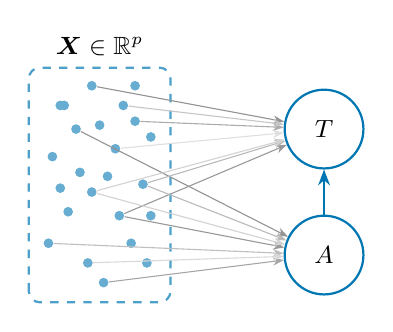
\begin{tikzpicture}[
  baseline=(current bounding box.center),
  xnode/.style={circle, fill=myaccent!60, minimum size=3.5pt, inner sep=0pt},
  bignode/.style={circle, draw=myaccent, thick, minimum size=10mm, font=\small, fill=white},
  arrbase/.style={-{Stealth[length=1.4mm]}, thin}
]
% Cluster of X covariates - deterministic positions
\foreach \i/\x/\y in {
  1/0.15/2.70, 2/0.55/2.95, 3/0.35/2.40, 4/0.05/2.05,
  5/0.75/1.80, 6/0.25/1.35, 7/0.00/0.95, 8/0.50/0.70,
  9/0.90/1.30, 10/1.10/2.50, 11/0.85/2.15, 12/0.20/2.70,
  13/1.20/1.70, 14/0.55/1.60, 15/1.05/0.95, 16/0.15/1.65,
  17/0.70/0.45, 18/1.25/0.70, 19/1.10/2.95, 20/0.65/2.45,
  21/0.40/1.85, 22/0.95/2.70, 23/1.30/2.30, 24/1.30/1.30
}{
  \node[xnode] (X\i) at (\x, \y) {};
}
% Group label
\node[font=\small] at (0.65, 3.45) {$\bm{X} \in \R^p$};
% Dashed border around X cluster
\draw[myaccent!70, dashed, thick, rounded corners=4pt]
  (-0.25, 0.20) rectangle (1.55, 3.18);
% A and T nodes on the right
\node[bignode] (A) at (3.5, 0.80) {$A$};
\node[bignode] (T) at (3.5, 2.40) {$T$};
% Arrows from X to A only
\foreach \i/\col in {3/gray!85, 17/gray!70, 7/gray!50, 8/gray!30}{
  \draw[arrbase, \col] (X\i) -- (A);
}
% Arrows from X to T only
\foreach \i/\col in {2/gray!85, 10/gray!65, 22/gray!45, 11/gray!25}{
  \draw[arrbase, \col] (X\i) -- (T);
}
% Confounders: arrows from X to BOTH A and T
\foreach \i/\col in {9/gray!80, 13/gray!55, 14/gray!35}{
  \draw[arrbase, \col] (X\i) -- (A);
  \draw[arrbase, \col] (X\i) -- (T);
}
% A -> T causal arrow
\draw[-{Stealth[length=2mm]}, thick, myaccent] (A) -- (T);
\end{tikzpicture}
\end{minipage}
\end{column}
\end{columns}
\end{frame}

%=========================================================
% PART 1 — The novelty, stated up front
%=========================================================
\section{What's new}

%---------------------------------------------------------
\begin{frame}{Novelties}
\begin{itemize}
  \item \textbf{Framework.} We bring the Bayesian Causal Forest (Hahn et al., 2020) to survival data.
  \vspace{0.7cm}
  \item \textbf{A new place to regularise a tree ensemble:} a \alert{horseshoe prior on the leaf step heights}, not the tree structure.
  \vspace{0.7cm}
  \item Non-conjugate $\Rightarrow$ tailored \alert{reversible-jump-within-Gibbs} sampler.
\end{itemize}
\end{frame}

%=========================================================
% PART 2 — Problem setup & model (slides from ISBA2026.tex)
%=========================================================
\section{Problem setup}

%---------------------------------------------------------
\begin{frame}{The setting}
\textbf{Potential outcomes.} For treatment $a \in \{0,1\}$, each patient has an event time $T_i(a)$ and a censoring time $C_i(a)$.

\vspace{0.3cm}

\textbf{Observational data} $(Y_i, \delta_i, A_i, X_i)$, $i = 1,\ldots,n$:
\begin{itemize}
  \item $A_i \in \{0,1\}$ \;(binary, non-randomised);\quad $X_i \in \R^p$ with $p \gg n$
  \item $Y_i = \min\bigl(T_i(A_i),\, C_i(A_i)\bigr)$,\;\; $\delta_i = \mathbf{1}\{T_i(A_i) \le C_i(A_i)\}$ \;(right-censored)
\end{itemize}

\vspace{0.8cm}

\textbf{Estimand.} The conditional average treatment effect (CATE) on the log-survival scale,
\[
\tau(x) \;:=\; \E\left[\log T(1) - \log T(0)\,\big|\, X = x\right].
\]
\begin{center}
{\footnotesize\color{black!55} Identifiable under standard causal assumptions.}
\end{center}
\end{frame}

%---------------------------------------------------------
\begin{frame}{An accelerated failure time decomposition}
We model the log-event times with an \textbf{accelerated failure time (AFT)} model:
\[
\log T(a) \;=\; f\bigl(x, \hat e(x)\bigr) \;+\; a \cdot \tau(x) \;+\; \varepsilon, \qquad \varepsilon \;\sim\; \N(0, \sigma^2).
\]

\begin{itemize}
  \item $f$: prognostic function.
  \item $\hat e(x)$: estimated propensity score.
  \item $\tau(x)$: heterogeneous treatment effect.
\end{itemize}
\bigskip

\textbf{Why AFT here?} AFT effects are collapsible: the marginal effect is the average of conditional effects.

\bigskip
\textbf{Plan.} Place a flexible Bayesian tree-ensemble prior on both $f$ and $\tau$, separately.
\end{frame}

%---------------------------------------------------------
\section{From BART to Horseshoe Forests}

\begin{frame}{BART in one slide}
\begin{center}
\begin{minipage}[c]{0.38\linewidth}
  \centering
  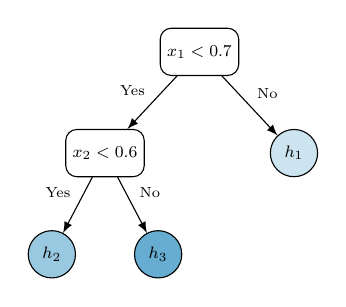
\begin{tikzpicture}[
        scale=0.75, transform shape,
        box/.style={rectangle, draw, rounded corners, align=center, minimum height=8mm, minimum width=13mm, font=\footnotesize},
        leaf/.style={circle, draw, align=center, minimum size=8mm, font=\footnotesize},
        line/.style={-latex}
    ]
    \node [box] (root) {$x_1 < 0.7$};
    \node [box, below=0.9cm of root, xshift=-1.6cm] (left) {$x_2 < 0.6$};
    \node [leaf, fill=myaccent!20, below=0.9cm of root, xshift=1.6cm] (h1) {$h_1$};
    \node [leaf, fill=myaccent!40, below=0.9cm of left, xshift=-0.9cm] (h2) {$h_2$};
    \node [leaf, fill=myaccent!60, below=0.9cm of left, xshift=0.9cm] (h3) {$h_3$};
    \draw[line] (root) -- (left) node[midway, above left, font=\scriptsize] {Yes};
    \draw[line] (root) -- (h1) node[midway, above right, font=\scriptsize] {No};
    \draw[line] (left) -- (h2) node[midway, above left, font=\scriptsize] {Yes};
    \draw[line] (left) -- (h3) node[midway, above right, font=\scriptsize] {No};
  \end{tikzpicture}
\end{minipage}\hfill
\begin{minipage}[c]{0.08\linewidth}
  \centering
  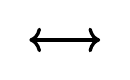
\begin{tikzpicture}
    \draw[<->, very thick] (0,0) -- (0.9,0);
  \end{tikzpicture}
\end{minipage}\hfill
\begin{minipage}[c]{0.38\linewidth}
  \centering
  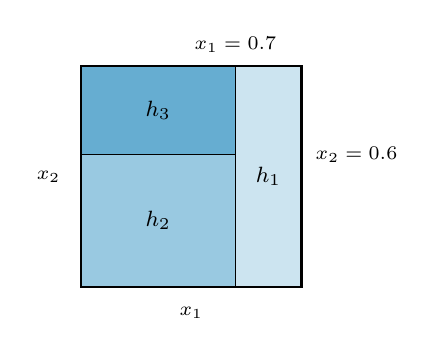
\begin{tikzpicture}[scale=2.8]
    \fill[myaccent!20] (0.7, 0) rectangle (1, 1);
    \fill[myaccent!40] (0, 0)   rectangle (0.7, 0.6);
    \fill[myaccent!60] (0, 0.6) rectangle (0.7, 1);
    \draw[thick] (0, 0) rectangle (1, 1);
    \draw[thin] (0.7, 0) -- (0.7, 1);
    \draw[thin] (0, 0.6) -- (0.7, 0.6);
    \node[below, font=\scriptsize] at (0.5, -0.05) {$x_1$};
    \node[left, font=\scriptsize] at (-0.05, 0.5) {$x_2$};
    \node[right, font=\scriptsize] at (1.02, 0.6) {$x_2 = 0.6$};
    \node[above, font=\scriptsize] at (0.7, 1.02) {$x_1 = 0.7$};
    \node[font=\footnotesize] at (0.85, 0.5) {$h_1$};
    \node[font=\footnotesize] at (0.35, 0.3) {$h_2$};
    \node[font=\footnotesize] at (0.35, 0.8) {$h_3$};
  \end{tikzpicture}
\end{minipage}
\end{center}


\vspace{-0.2em}

\textbf{Model.} $g(x) = \sum_{j=1}^{m} g(x;\, \T_j, \Hh_j)$ --- a sum of many shallow trees, each piecewise constant on a partition of the covariate space.

\vspace{0.3cm}

\textbf{Prior.}
\begin{itemize}
  \item Tree shape $\T_j$: depth-penalised Galton--Watson.
  \item Step heights $\Hh_j$: i.i.d.\ Gaussian, variance $\propto 1/m$.
\end{itemize}

\end{frame}

%---------------------------------------------------------
\begin{frame}{Where does regularisation come from in BART?}
Two places to regularise a tree ensemble:

\bigskip

\begin{enumerate}
  \item \textbf{Via the tree structure} $\T_j$ --- depth penalty, splitting rules, covariate selection (DART [Linero, 2018], Soft-BART, \ldots).
  \medskip
  \item \textbf{Via the step heights} $\Hh_j$ --- shrink the \emph{magnitudes} of step heights.
\end{enumerate}

\bigskip

Existing work focuses on (1), but controlling tree structure alone is not enough in high dimensions, or induces bias by dropping relevant confounders.
\bigskip

\textbf{Novel contribution.} Regularise through (2): a global--local shrinkage prior on the step heights.
\end{frame}

%---------------------------------------------------------
\begin{frame}{Horseshoe prior on the step heights}
\begin{columns}[T,onlytextwidth]
\begin{column}{0.55\textwidth}
For a tree with step heights $\ell = 1,\ldots, L$:
\[
h_\ell \mid \lambda_\ell^2, \gamma^2 \;\sim\; \N\bigl(0,\, \lambda_\ell^2\, \gamma^2\bigr),
\]
\[
\lambda_\ell \;\sim\; \mathcal{C}^+(0, 1), \qquad \gamma \;\sim\; \mathcal{C}^+(0, 1).
\]

\vspace{0.8cm}

\textbf{Global--local shrinkage:}
\begin{itemize}
  \item $\gamma$ pulls \emph{everything} to zero.
  \item $\lambda_\ell$ lets individual step heights \emph{escape} locally.
\end{itemize}

\smallskip
\textit{$\Rightarrow$ regularise globally, pick up signals locally.}
\end{column}
\begin{column}{0.50\textwidth}
\centering
\vspace{0.3cm}
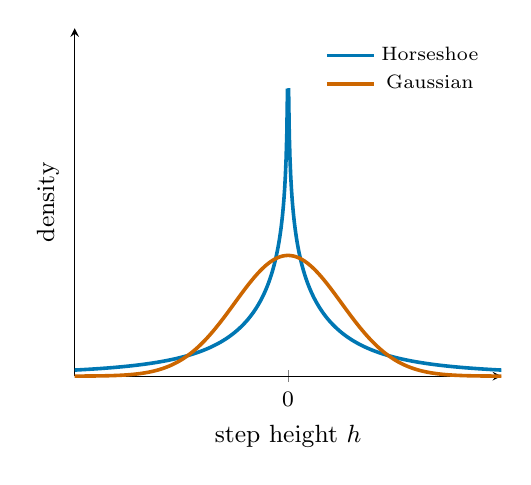
\begin{tikzpicture}
\begin{axis}[
  width=7.0cm, height=6.0cm,
  xlabel={step height $h$}, ylabel={density},
  xmin=-4, xmax=4, ymin=0, ymax=1.15,
  ytick=\empty, xtick={0},
  axis lines=left, clip=false,
  legend style={font=\scriptsize, draw=none, fill=none,
                at={(0.98,0.98)}, anchor=north east},
  label style={font=\small},
  tick label style={font=\footnotesize},
]
% Horseshoe: pole at 0 + heavy tails (accent)
\addplot[domain=0.01:4, samples=300, line width=1.3pt, myaccent]
  {ln(1 + 4/(x*x)) / (2*3.14159^1.5)};
\addlegendentry{Horseshoe}
\addplot[domain=-4:-0.01, samples=300, line width=1.3pt, myaccent, forget plot]
  {ln(1 + 4/(x*x)) / (2*3.14159^1.5)};
% Gaussian: light-tailed bell (dark orange)
\addplot[domain=-4:4, samples=200, line width=1.3pt, orange!80!black]
  {0.3989*exp(-x*x/2)};
\addlegendentry{Gaussian}
\end{axis}
\end{tikzpicture}
\end{column}
\end{columns}
\end{frame}

%=========================================================
% OLD v1 SLIDES — commented out, replaced by the ISBA2026.tex slides above
%=========================================================
\iffalse

%---------------------------------------------------------
\begin{frame}{The problem has three ingredients}
\vspace{0.2cm}
\begin{center}
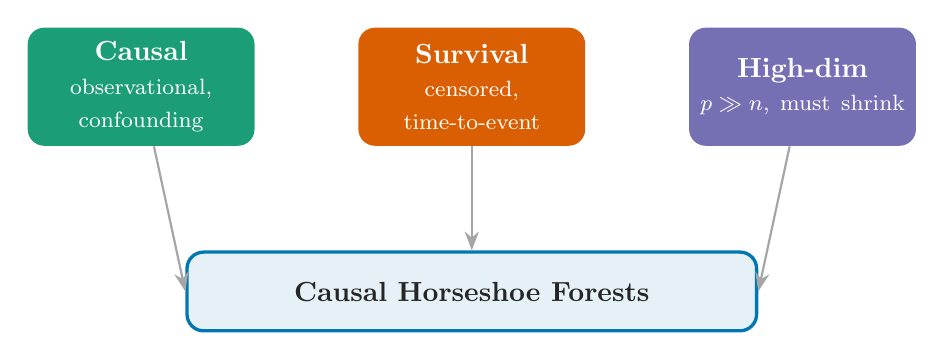
\begin{tikzpicture}[
  ingbox/.style={rounded corners=6pt, text width=2.6cm, minimum height=1.5cm,
              align=center, text=white, font=\bfseries, inner sep=4pt},
  arr/.style={-{Stealth[length=2.4mm]}, thick, gray!70}
]
\node[ingbox, fill=causalcol]   (c) at (-4.2, 0) {Causal\\ {\footnotesize\mdseries observational, confounding}};
\node[ingbox, fill=survivalcol] (s) at ( 0.0, 0) {Survival\\ {\footnotesize\mdseries censored, time-to-event}};
\node[ingbox, fill=highdimcol]  (h) at ( 4.2, 0) {High-dim\\ {\footnotesize\mdseries $p \gg n$, must shrink}};

\node[draw=myaccent, very thick, rounded corners=6pt, fill=myaccent!10,
      text width=7.0cm, minimum height=1.0cm, align=center, font=\bfseries,
      text=black!85] (m) at (0,-2.6)
      {Causal Horseshoe Forests};

\draw[arr] (c) -- (m.west);
\draw[arr] (s) -- (m.north);
\draw[arr] (h) -- (m.east);
\end{tikzpicture}
\end{center}
\end{frame}

%---------------------------------------------------------
\begin{frame}{Ingredient 1 --- Causal}
\ingbar{1}{0}{0}
\begin{columns}[T,onlytextwidth]
\begin{column}{0.60\textwidth}
\vspace{0.2cm}
\textbf{Observational:} $A$ not randomised $\Rightarrow$ $A,T$ share causes.

\bigskip

\textbf{Standard identifying assumptions} (SUTVA, unconfoundedness, positivity, independent censoring).

\bigskip

\textbf{Estimand --- CATE} on the log scale:
\[
\tau(x) \;:=\; \E\!\left[\log T(1) - \log T(0)\,\big|\, \bm X = x\right].
\]

\bigskip

A dropped covariate may be a confounder $\Rightarrow$ \alert{keep every covariate.}
\end{column}
\begin{column}{0.38\textwidth}
\centering
\vspace{0.4cm}
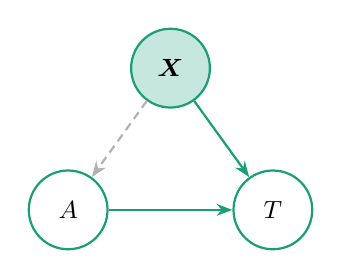
\begin{tikzpicture}[
  every node/.style={circle, draw=causalcol, thick, minimum size=1cm, font=\small},
  arr/.style={-{Stealth[length=2mm]}, thick, causalcol}
]
\node[fill=causalcol!25] (X) at (0,1.4)    {$\bm{X}$};
\node (A) at (-1.3,-0.4) {$A$};
\node (T) at (1.3,-0.4)  {$T$};
\draw[arr, gray!60, densely dashed] (X) -- (A);
\draw[arr] (X) -- (T);
\draw[arr] (A) -- (T);
\end{tikzpicture}

\bigskip
{\footnotesize Conditioning on $\bm X$ closes the back-door path.}
\end{column}
\end{columns}
\end{frame}

%---------------------------------------------------------
\begin{frame}{Ingredient 2 --- Survival}
\ingbar{0}{1}{0}
\begin{columns}[T,onlytextwidth]
\begin{column}{0.54\textwidth}
\vspace{0.1cm}
Right-censored outcome; \textbf{accelerated failure time (AFT)} model for $\log T$:
\[
\log T(a) = \underbrace{f\bigl(x, \hat e(x)\bigr)}_{\text{prognostic}}
            + \underbrace{a\cdot \tau(x)}_{\text{treatment}}
            + \varepsilon,\quad \varepsilon\sim\N(0,\sigma^2).
\]

\smallskip
\begin{itemize}
  \item BCF structure (Hahn et al., 2020): separate forests for $f,\tau$; propensity $\hat e(x)$ enters $f$.
  \item $e^{\tau(x)}$ = \emph{acceleration factor}: collapsible, interpretable.
\end{itemize}
\end{column}
\begin{column}{0.46\textwidth}
\centering
\vspace{0.2cm}
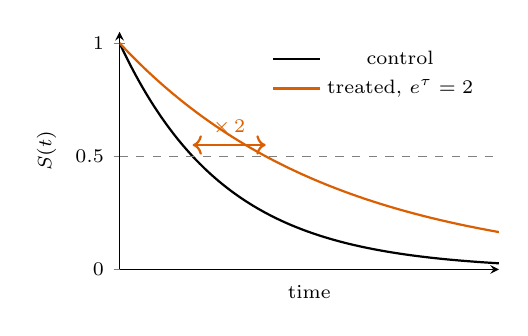
\begin{tikzpicture}
\begin{axis}[
  width=6.4cm, height=4.6cm,
  xlabel={time}, ylabel={$S(t)$},
  xmin=0, xmax=12, ymin=0, ymax=1.05,
  xtick=\empty, ytick={0,0.5,1},
  legend pos=north east,
  legend style={font=\scriptsize, draw=none},
  axis lines=left,
  tick label style={font=\scriptsize},
  label style={font=\scriptsize},
]
\addplot[domain=0:12, samples=200, thick, black]      {exp(-0.30*x)};
\addlegendentry{control}
\addplot[domain=0:12, samples=200, thick, survivalcol]{exp(-0.15*x)};
\addlegendentry{treated, $e^{\tau}=2$}
\draw[dashed, gray] (axis cs:0,0.5) -- (axis cs:12,0.5);
\draw[<->, thick, survivalcol]
  (axis cs:2.31,0.55) -- (axis cs:4.62,0.55)
  node[midway,above,font=\scriptsize,text=survivalcol]{$\times\,2$};
\end{axis}
\end{tikzpicture}

{\footnotesize $e^{\tau(x)}=2 \Rightarrow$ median survival doubles.}
\end{column}
\end{columns}
\end{frame}

%---------------------------------------------------------
\begin{frame}{Ingredient 3 --- High-dimensional}
\ingbar{0}{0}{1}
With $p \gg n$, must regularise. \textbf{BART} = sum of $m$ shallow trees:
\[
g(x) = \sum_{j=1}^m g(x;\,\T_j,\Hh_j).
\]

\bigskip

\textbf{Two places to regularise:}
\begin{enumerate}
  \item \textbf{Tree structure} $\T_j$ --- DART, Soft-BART, Shrinkage BCF.
  \item \textbf{Step heights} $\Hh_j$ --- shrink the \emph{magnitudes}.
\end{enumerate}

\bigskip

Existing work does (1); selecting splits can drop a weak confounder.

\smallskip
\alert{Our move: regularise through (2) --- every covariate stays split-eligible.}
\end{frame}

%=========================================================
% PART 3 — Our solution
%=========================================================
\section{Our solution}

%---------------------------------------------------------
\begin{frame}{Horseshoe prior on the step heights}
\begin{columns}[T,onlytextwidth]
\begin{column}{0.58\textwidth}
\vspace{0.2cm}
For a tree $\T$ with leaves $\ell = 1,\ldots,L$:
\[
h_\ell \mid \lambda_\ell^2,\gamma^2 \;\sim\; \N\bigl(0,\,\lambda_\ell^2\,\gamma^2\bigr),
\]
\[
\lambda_\ell \sim \mathcal{C}^+(0,1), \qquad \gamma \sim \mathcal{C}^+(0,1).
\]

\bigskip

\textbf{Two defining features:}
\begin{itemize}
  \item \alert{Pole at zero} --- strong shrinkage of noise.
  \item \alert{Heavy tails} --- large signals are not shrunk.
\end{itemize}

\bigskip

\textbf{Global--local:} $\gamma$ shrinks \emph{everything};
$\lambda_\ell$ lets individual leaves \emph{escape}.
\end{column}
\begin{column}{0.42\textwidth}
\centering
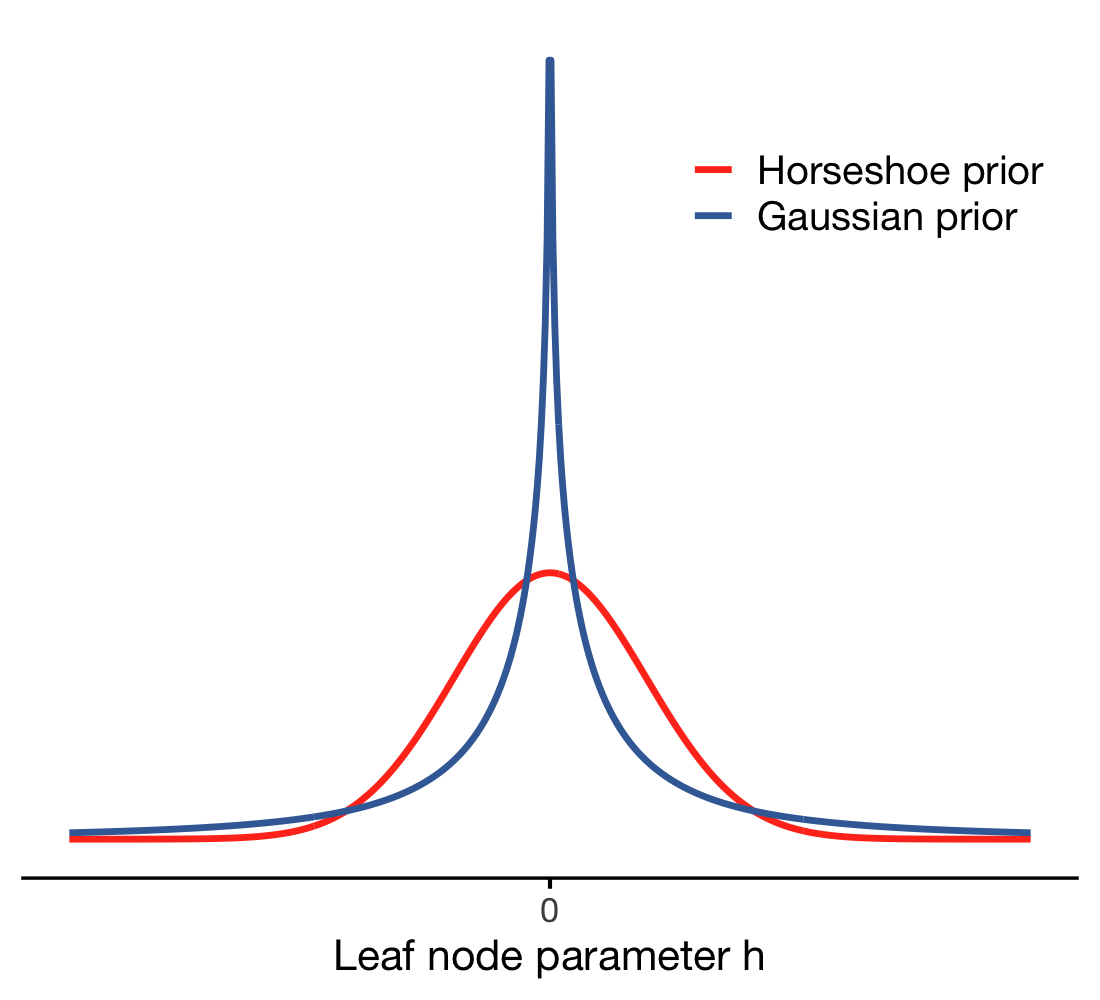
\includegraphics[width=\linewidth]{Horseshoe_plot_ICSDS.png}
\end{column}
\end{columns}
\end{frame}

%---------------------------------------------------------
\begin{frame}{Why horseshoe beats DART}
\textbf{DART} (Linero, 2018): a Dirichlet prior on the \emph{splitting probabilities} of covariates.

\bigskip

\begin{columns}[T,onlytextwidth]
\begin{column}{0.34\textwidth}
Many covariates get near-zero posterior inclusion probability.

\bigskip

Dropping a (weak) confounder $\Rightarrow$ \alert{regularisation-induced confounding} (Hahn et al., 2020).
\end{column}
\begin{column}{0.60\textwidth}
\centering
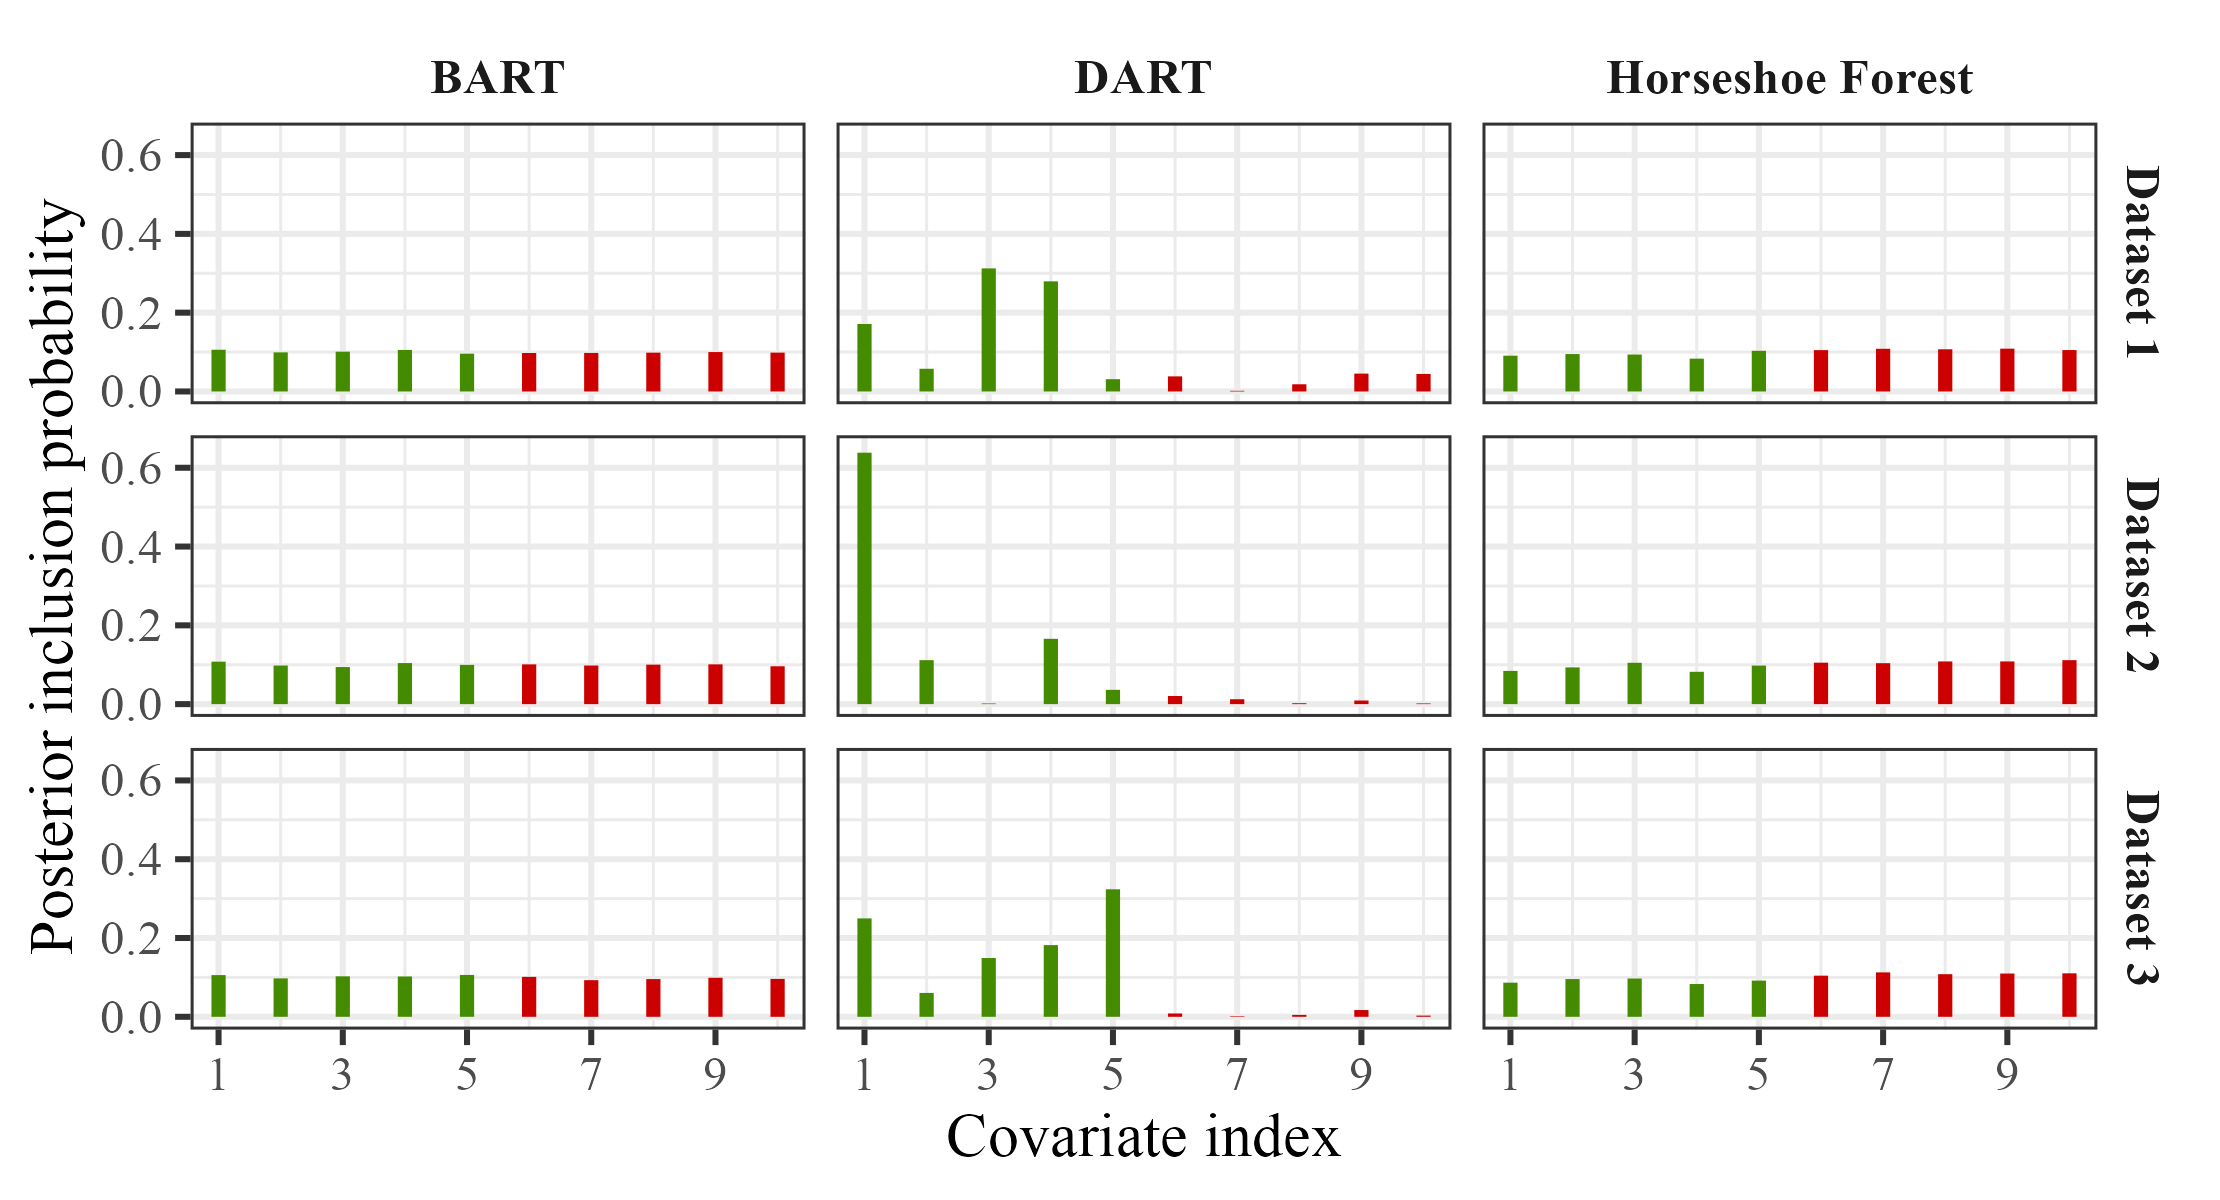
\includegraphics[width=\linewidth]{revision_posterior_inclusion_plot.png}\\
{\footnotesize Posterior inclusion probabilities; DART can concentrate on the \emph{wrong} subset.}
\end{column}
\end{columns}

\bigskip

\alert{Horseshoe forest: keep every covariate split-eligible; shrink the \emph{magnitudes} instead.}
\end{frame}

\fi
%=========================================================
% END OLD v1 SLIDES
%=========================================================

%=========================================================
% PART 3 — Posterior inference
%=========================================================
\section{Posterior inference}

%---------------------------------------------------------
\begin{frame}{Inference: reversible-jump within Gibbs}
\begin{columns}[c,onlytextwidth]
\begin{column}{0.40\textwidth}
Non-conjugate $\Rightarrow$ step heights can't be marginalised out.

\vspace{1cm}

GROW / PRUNE change the dimension of $\Hh_j$ $\Rightarrow$ \alert{reversible-jump} proposal for $(\T_j,\Hh_j)$.

\vspace{1cm}

Outer Gibbs sampler: $f$, $\tau$, $\sigma^2$, augmented censored times (Tanner \& Wong, 1987).
\end{column}
\begin{column}{0.58\textwidth}
\centering
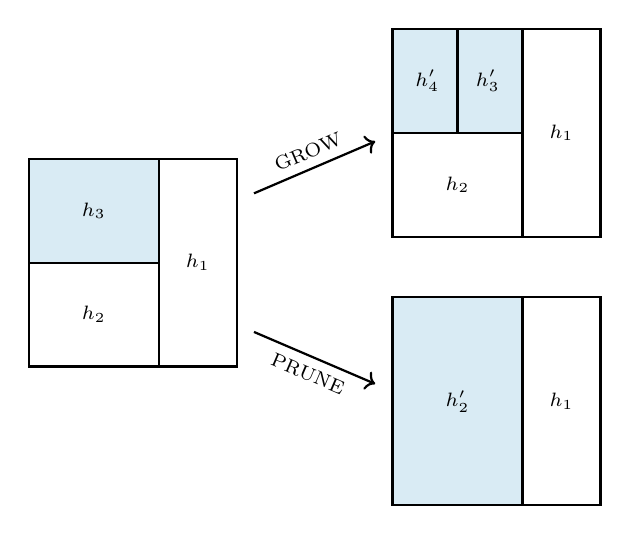
\begin{tikzpicture}[scale=1.1, every node/.style={font=\scriptsize}]
% Parent partition
\fill[myaccent!15] (0,1.2) rectangle (1.5,2.4);
\draw[thick] (0,0) rectangle (2.4,2.4);
\draw[thick] (1.5,0) -- (1.5,2.4);
\draw[thick] (0,1.2) -- (1.5,1.2);
\node at (0.75,1.8) {$h_3$};
\node at (0.75,0.6) {$h_2$};
\node at (1.95,1.2) {$h_1$};

\draw[->, thick] (2.6,2.0) -- (4.0,2.6) node[midway, above, sloped] {GROW};
\draw[->, thick] (2.6,0.4) -- (4.0,-0.2) node[midway, below, sloped] {PRUNE};

% GROW result
\begin{scope}[shift={(4.2,1.5)}]
\fill[myaccent!15] (0,1.2) rectangle (1.5,2.4);
\draw[thick] (0,0) rectangle (2.4,2.4);
\draw[thick] (1.5,0) -- (1.5,2.4);
\draw[thick] (0,1.2) -- (1.5,1.2);
\draw[thick] (0.75,1.2) -- (0.75,2.4);
\node at (0.4,1.8) {$h'_4$};
\node at (1.1,1.8) {$h'_3$};
\node at (0.75,0.6) {$h_2$};
\node at (1.95,1.2) {$h_1$};
\end{scope}

% PRUNE result
\begin{scope}[shift={(4.2,-1.6)}]
\fill[myaccent!15] (0,0) rectangle (1.5,2.4);
\draw[thick] (0,0) rectangle (2.4,2.4);
\draw[thick] (1.5,0) -- (1.5,2.4);
\node at (0.75,1.2) {$h'_2$};
\node at (1.95,1.2) {$h_1$};
\end{scope}
\end{tikzpicture}
\end{column}
\end{columns}
\end{frame}





\section{Simulations}

\begin{frame}{Simulation 1: CATE estimation as $p$ grows}
Non-linear treatment effect with sparse main (5\%) + interaction (1\%)  structure; $n = 200$, $p \in [50, 5000]$, censoring $\approx 35\%$.

\pause
\vspace{-0.3em}
\begin{center}
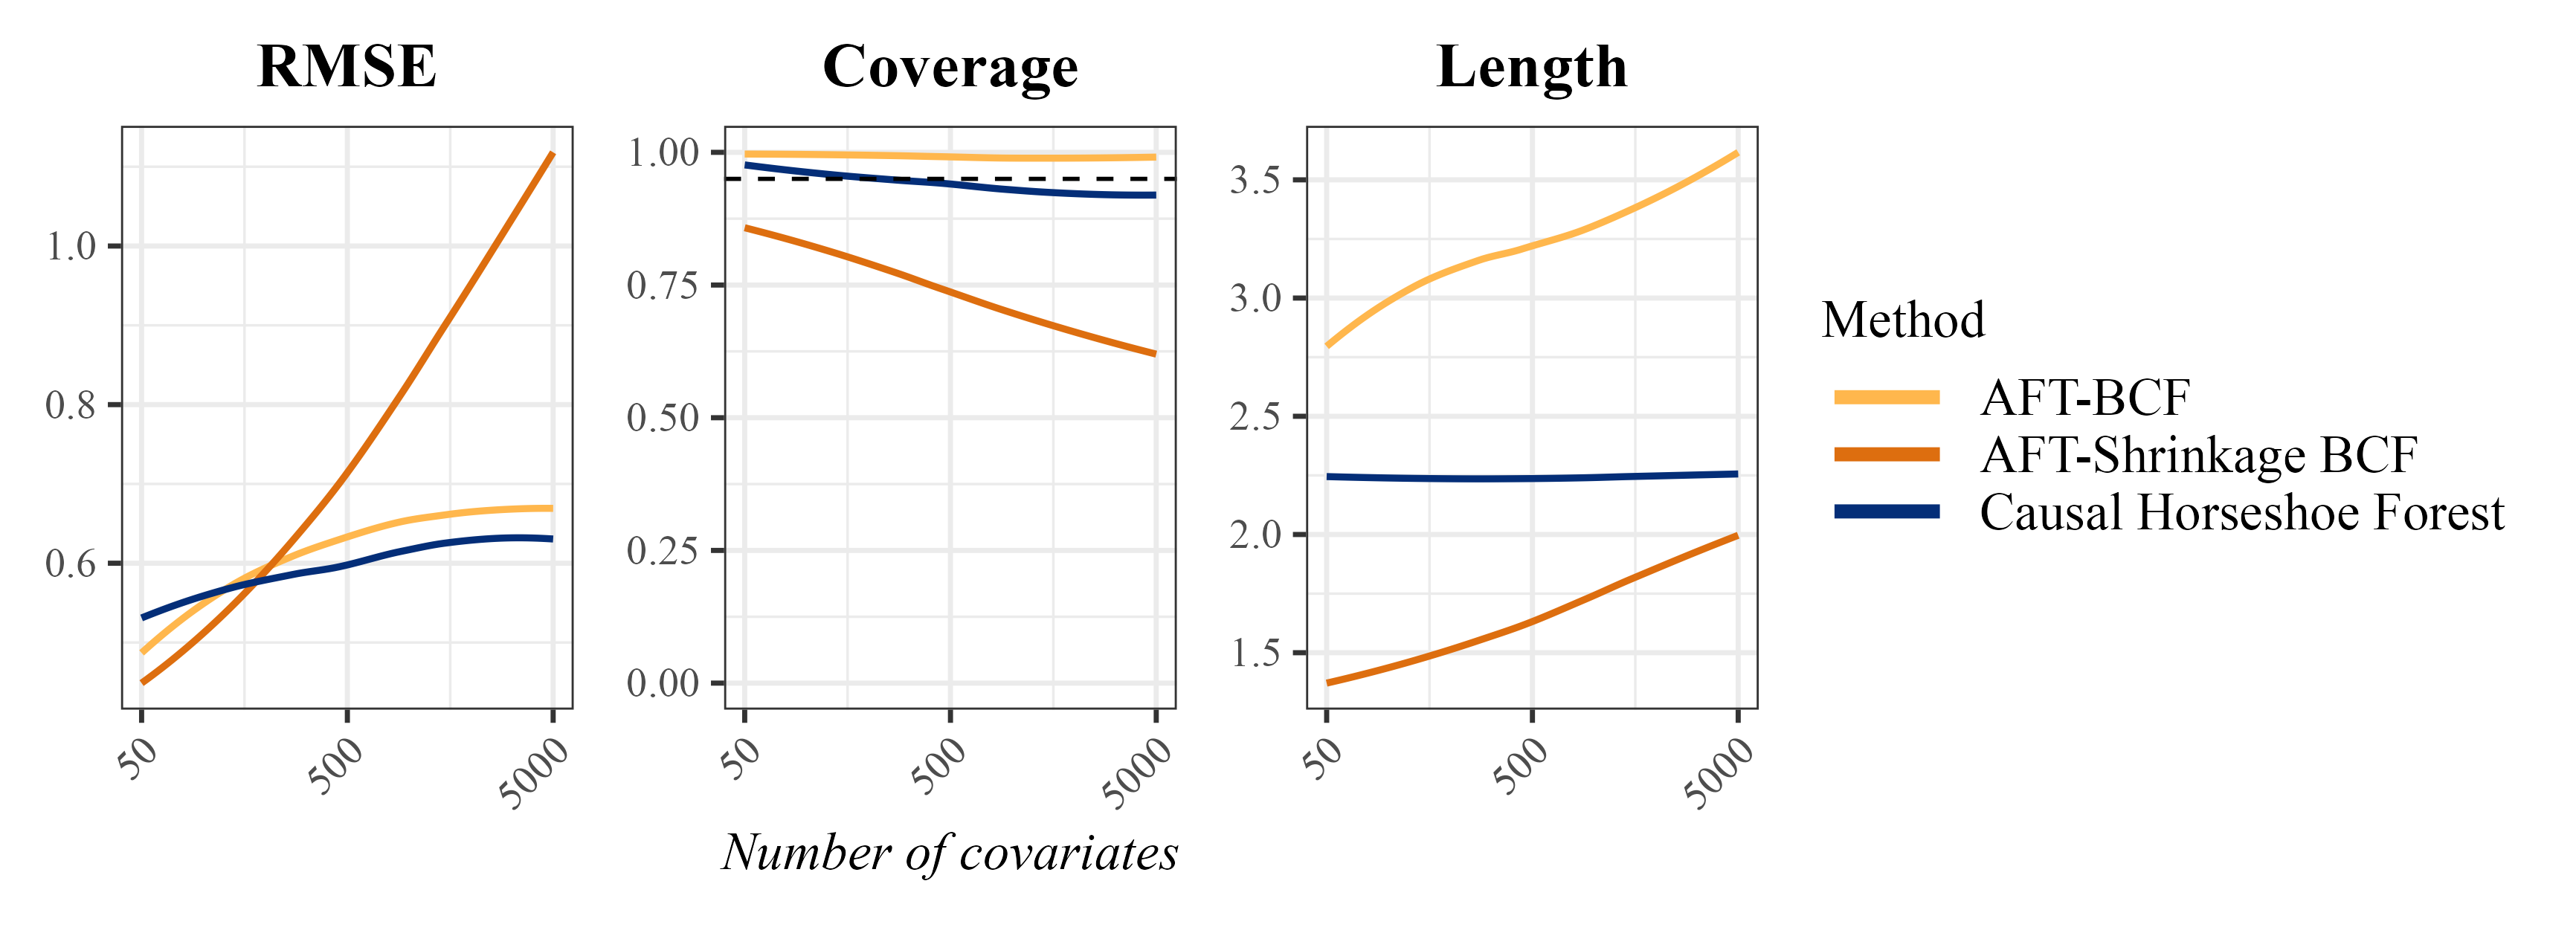
\includegraphics[width=0.95\linewidth]{revision_main_deeper.png}
\end{center}
\end{frame}

%---------------------------------------------------------
\begin{frame}{Simulation 2: regularisation-induced confounding}
$n = 100$, $p = 500$, censoring $\approx 35\%$. Two groups of confounders:
\begin{itemize}
  \item $|S| = 5$ \textbf{strong} confounders --- contribute substantially to both treatment and outcome.
  \item $|W| \in \{1, \ldots, 20\}$ \textbf{weak} confounders --- predict treatment, but contribute only weakly to the outcome.
\end{itemize}

\pause



\vspace{0.2cm}
\begin{center}
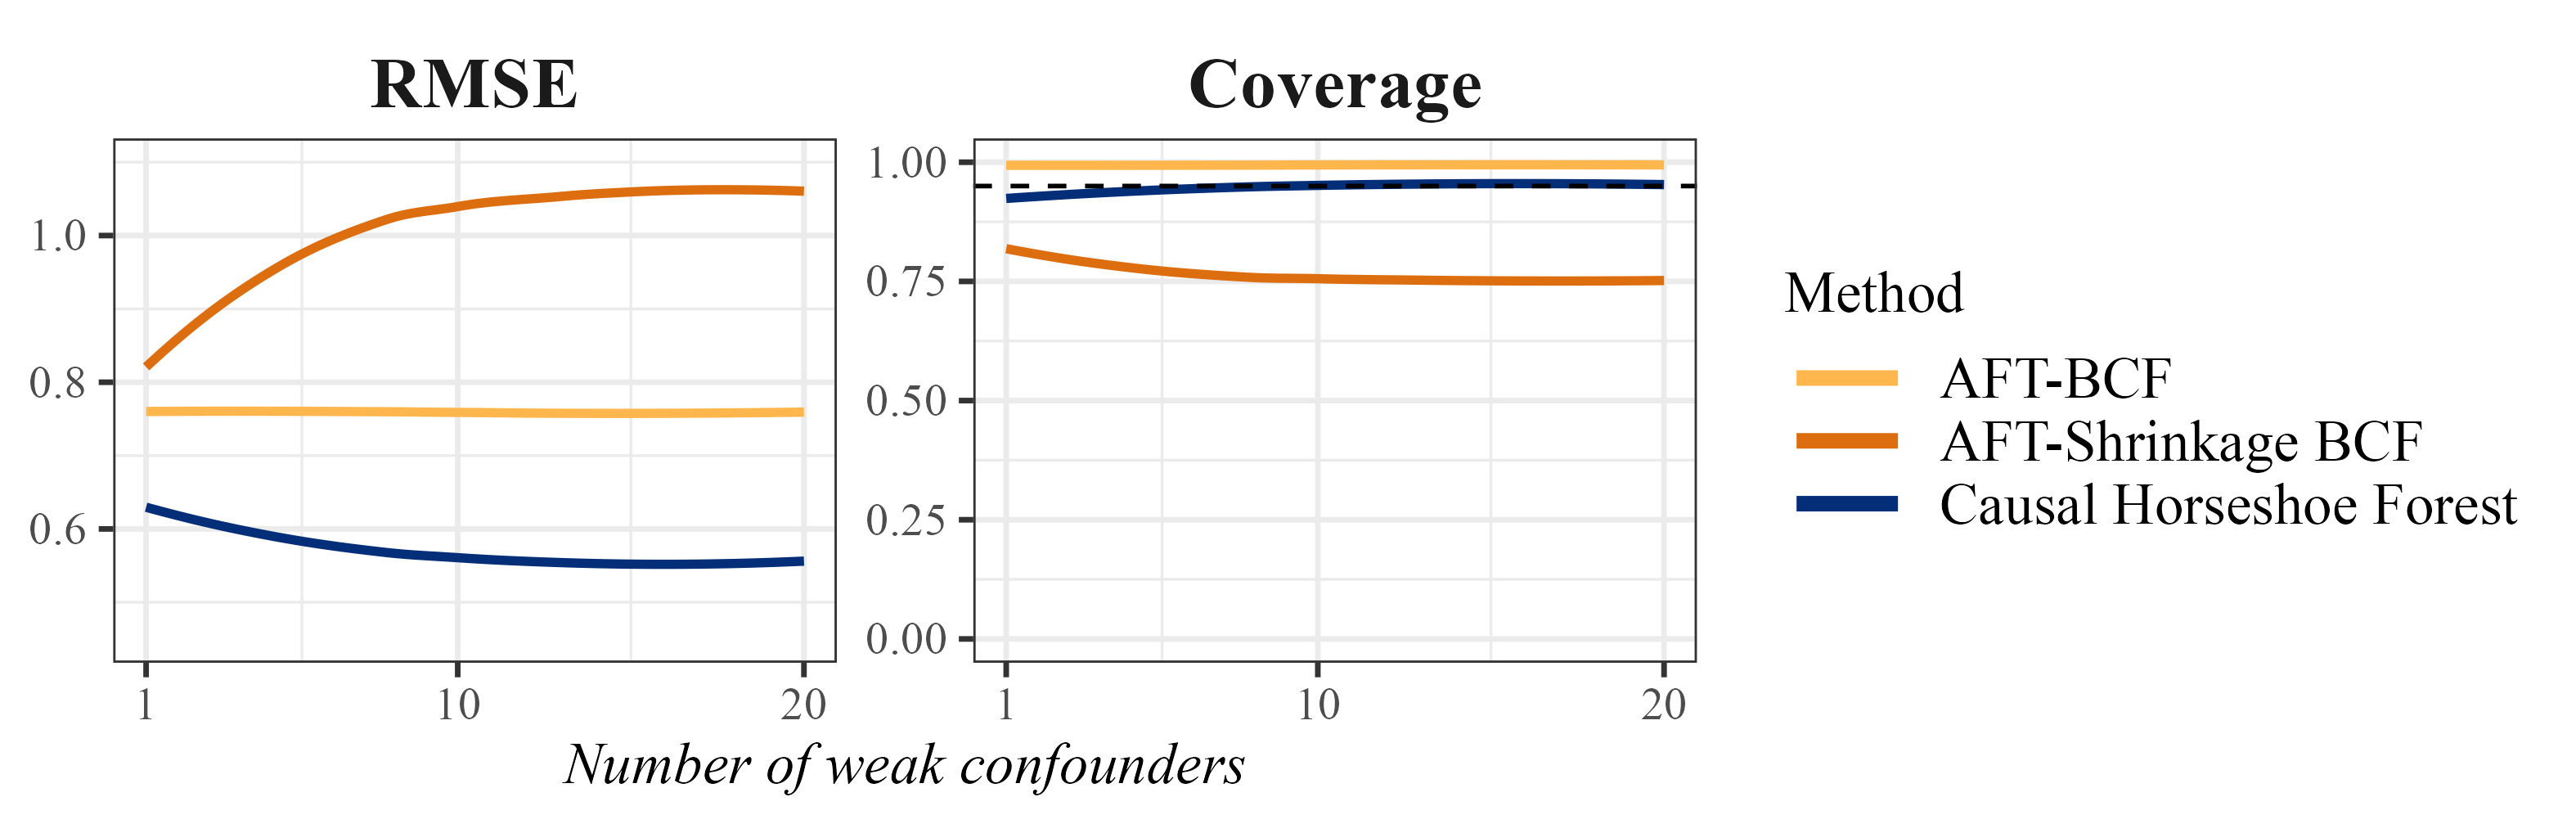
\includegraphics[width=0.95\linewidth]{revision_ric.png}
\end{center}
\end{frame}

%---------------------------------------------------------
\section{Application: pancreatic cancer}

\begin{frame}{Adjuvant radiotherapy in PDAC}
\begin{columns}[T,onlytextwidth]
\begin{column}{0.40\textwidth}
\textbf{Data.} TCGA-PAAD, $n = 110$ resected PDAC patients (6-month landmark).
\begin{itemize}
  \item \textit{Outcome}: overall survival; censoring $\approx 47\%$, median follow-up 23.3 mo.
  \item \textit{Treatment}: adjuvant radiotherapy.
  \item \textit{Covariates}: 11 clinical $+$ driver genes $+$ 3{,}000 most variable genes ($p \approx 3{,}029$).
\end{itemize}
\end{column}
\begin{column}{0.60\textwidth}
\centering
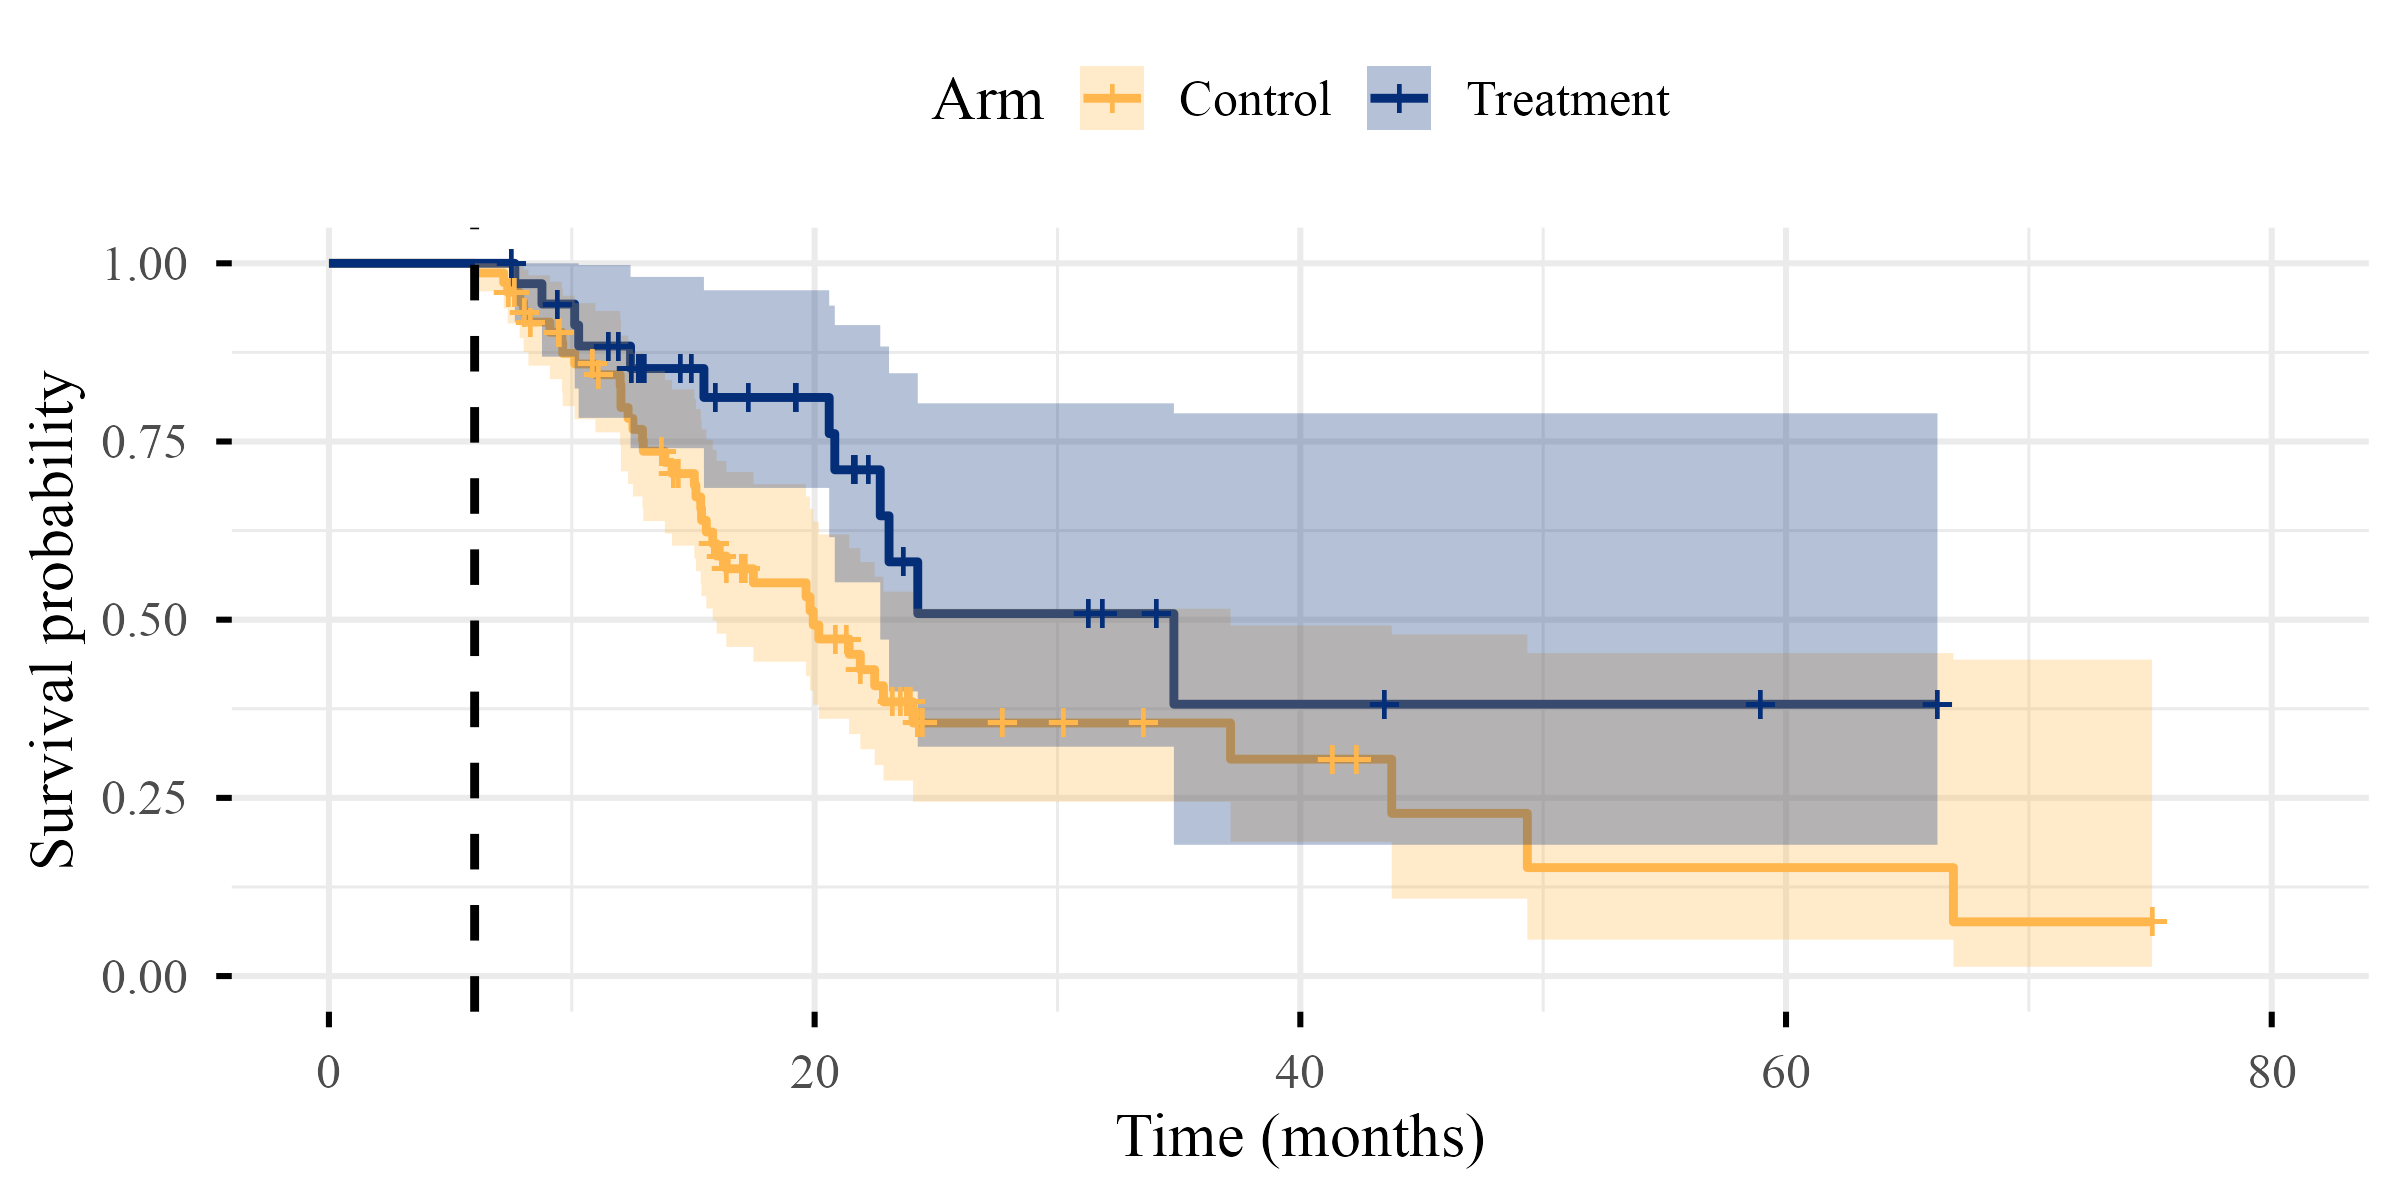
\includegraphics[width=\linewidth]{KM_Landmark.png}
\end{column}
\end{columns}


\bigskip

\textbf{Question.} Does adjuvant radiotherapy improve survival, and is the effect heterogeneous?

\end{frame}

%---------------------------------------------------------
\begin{frame}{Adjuvant radiotherapy in PDAC}
\begin{columns}[c,onlytextwidth]
\begin{column}{0.5\textwidth}
\centering
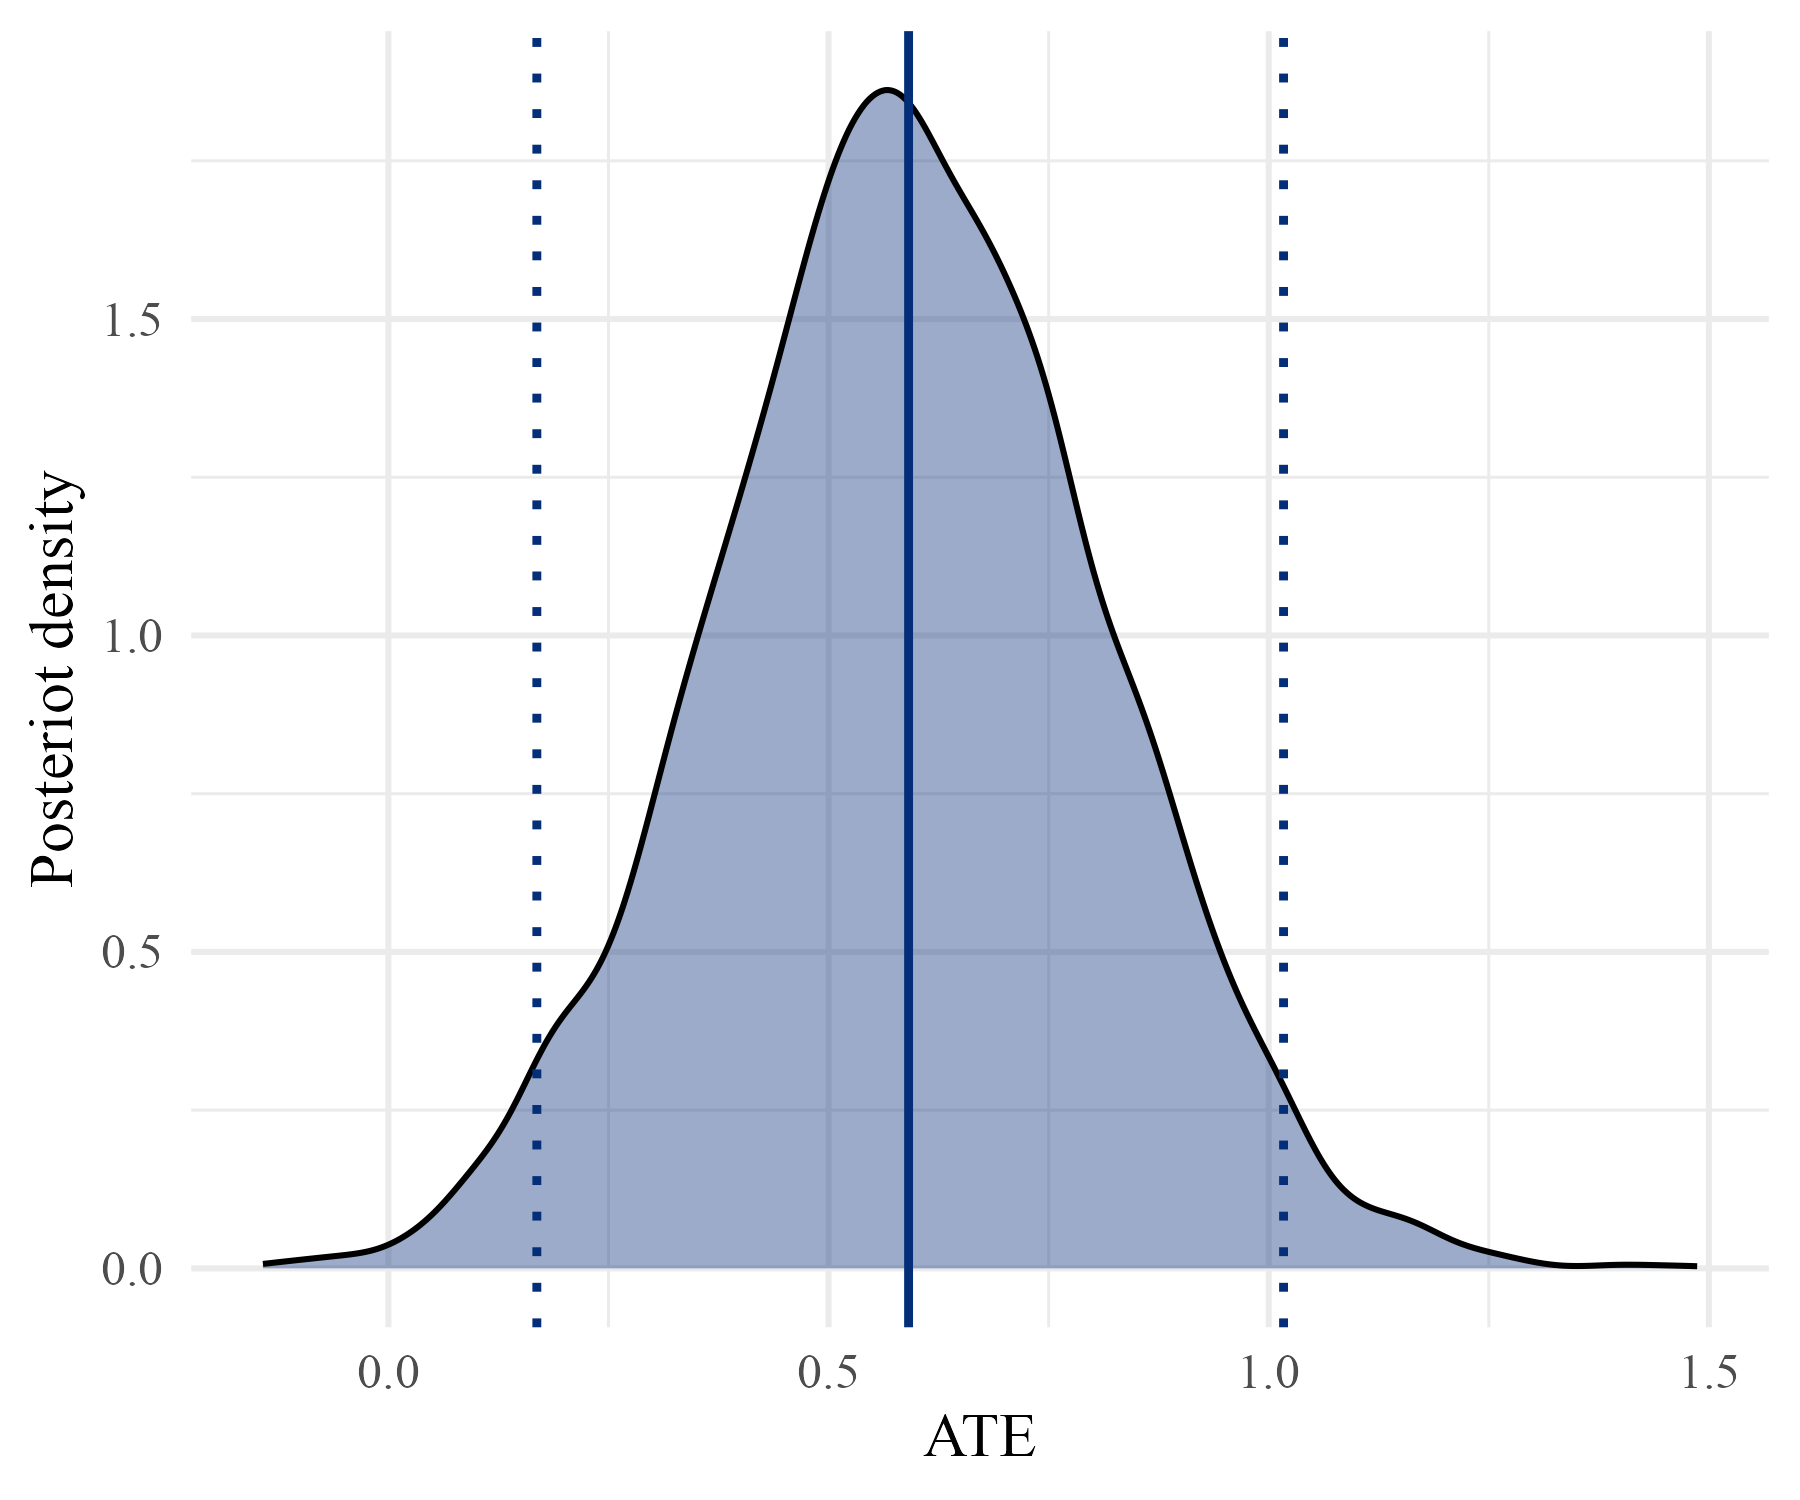
\includegraphics[width=\linewidth]{Plot_posteriorATE_Landmark.png}

\smallskip
{\footnotesize $\widehat{\text{ATE}} \approx 0.55$, \, 95\% CrI $(0.10,\, 1.02)$; \, acceleration factor $e^{0.55} \approx 1.73$.}
\end{column}
\begin{column}{0.5\textwidth}
\centering
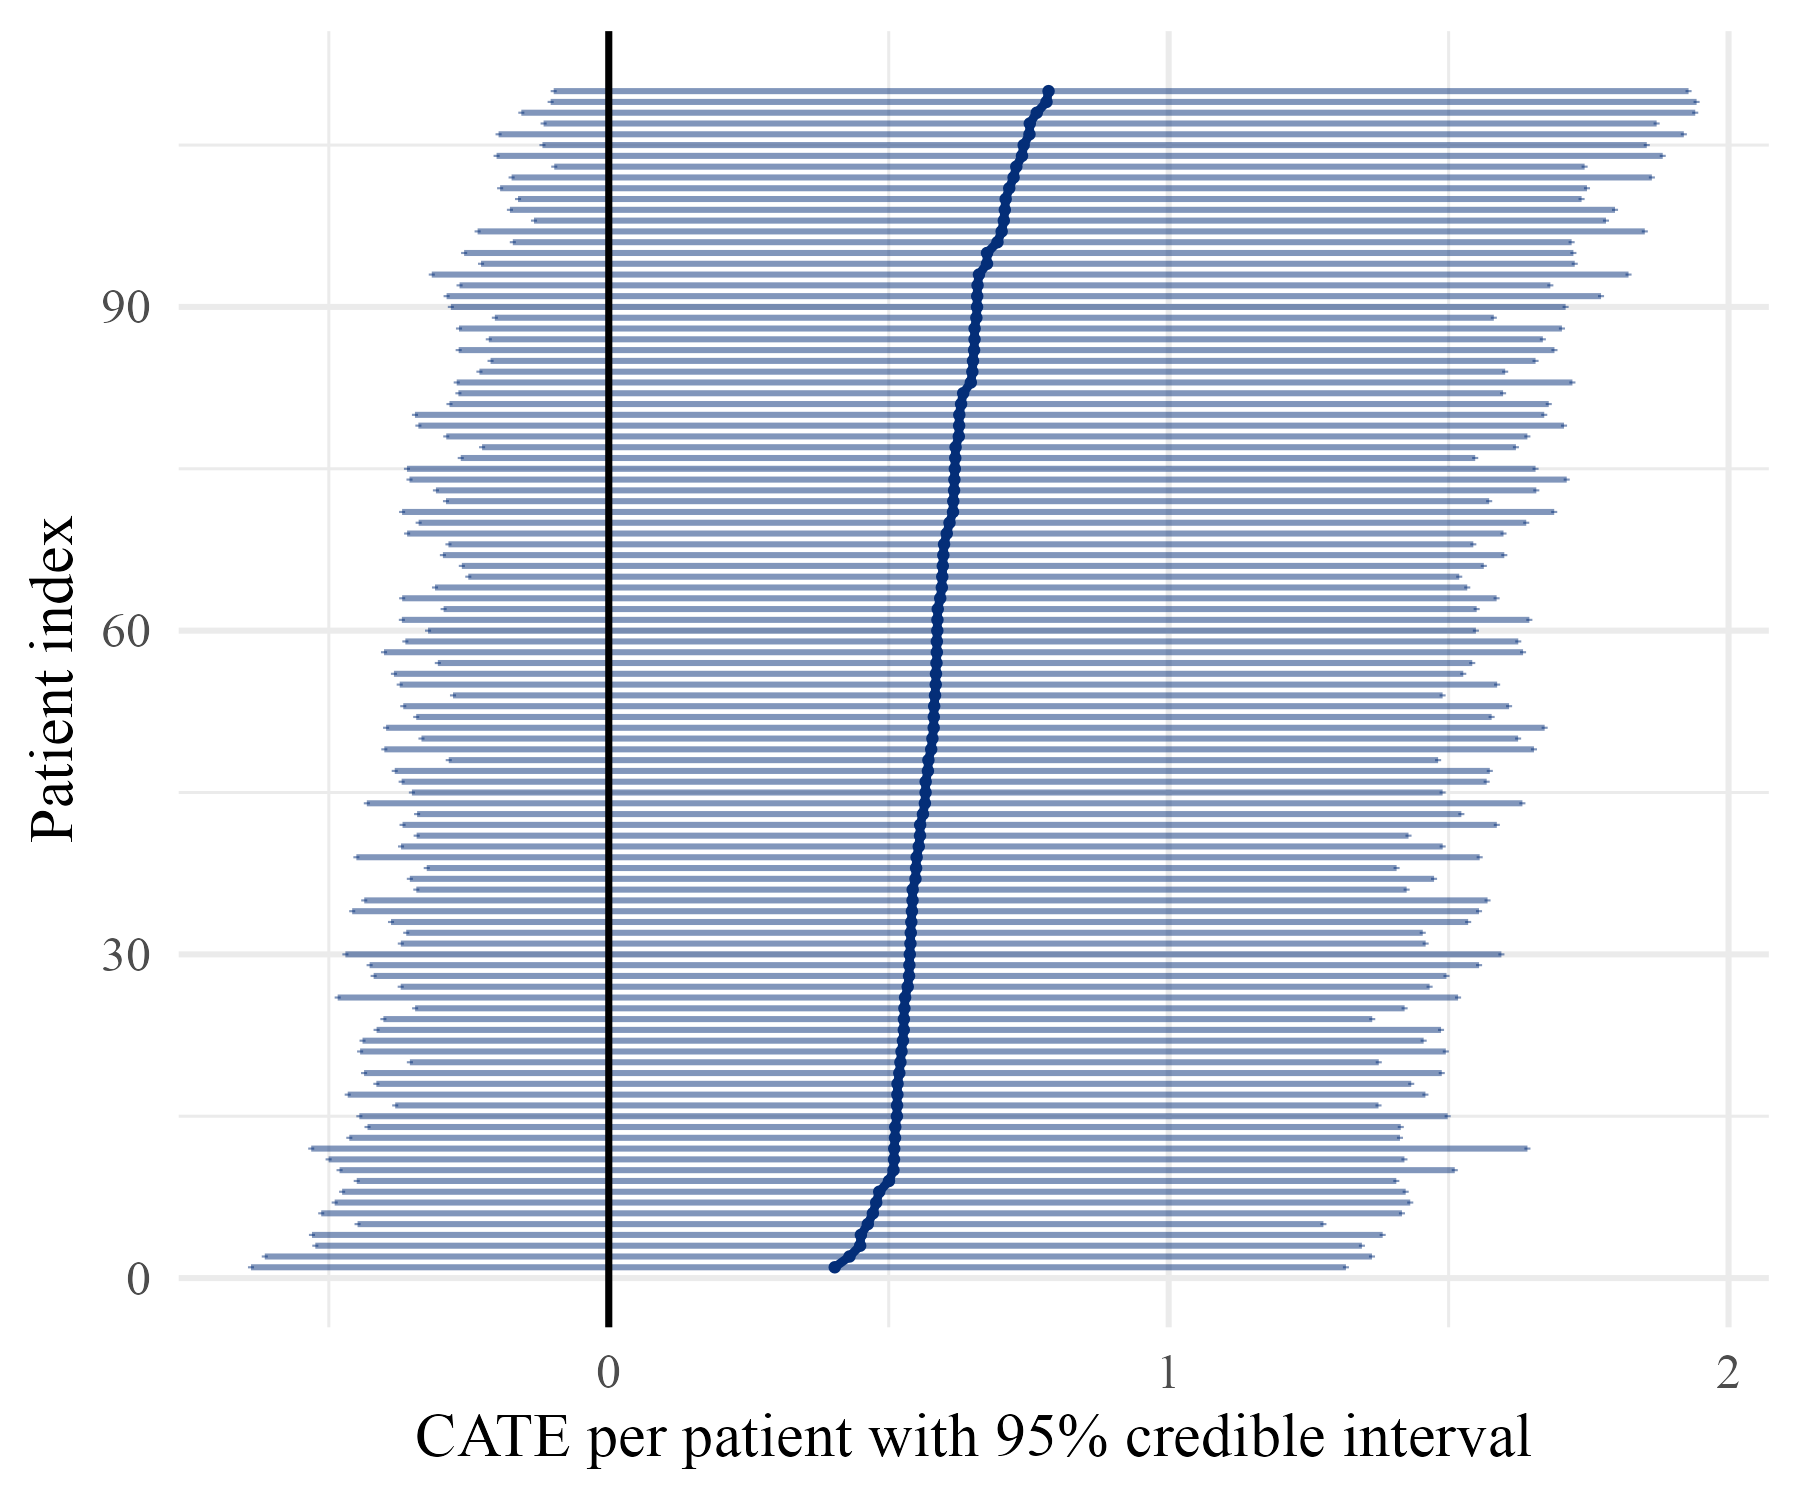
\includegraphics[width=\linewidth]{plot_CATEpatient_Landmark.png}

\smallskip
{\footnotesize Predictive performance: concordance index $= 0.75$.}
\end{column}
\end{columns}
\end{frame}




%=========================================================
% PART 5 — Wrap-up
%=========================================================
\section{Wrap-up}

%---------------------------------------------------------

\begin{frame}{Take-aways}
\begin{itemize}
\item \textbf{Where you regularise matters.} Shifting the regularisation from the tree structure onto the \emph{step heights} of a tree ensemble gives a flexible, adaptive prior for high-dimensional CATE estimation.  \vspace{0.7cm}
  \item \textbf{The price is a reversible-jump sampler.} A tailored tree proposal keeps the chain mixing well.
  \vspace{0.7cm}
  \item \textbf{Strong empirical performance.} Stable RMSE and near-nominal coverage as $p$ grows; robust to regularisation-induced confounding where competing methods break down.
\end{itemize}
\end{frame}

%---------------------------------------------------------
\begin{frame}{Thanks for your attention!}
\vspace{0.4cm}
\begin{columns}[T,onlytextwidth]

% ---- Left: Paper icon ----
\begin{column}{0.33\textwidth}
\centering
\begin{minipage}[t][2.6cm][c]{\linewidth}\centering

\begin{tikzpicture}[scale=0.95]
\fill[white] (0, 0) rectangle (1.6, 2.2);
\draw[myaccent, thick] (0, 0) rectangle (1.6, 2.2);
\fill[myaccent] (0, 1.85) rectangle (1.6, 2.2);
\draw[white, line width=0.8pt] (0.2, 2.025) -- (1.4, 2.025);
\foreach \y in {1.6, 1.4, 1.2, 1.0, 0.8, 0.6, 0.4} {
  \draw[gray!50, thick] (0.15, \y) -- (1.45, \y);
}
\fill[white] (1.25, 0.4) circle (0.32);
\draw[green!55!black, line width=2pt, line cap=round]
  (1.08, 0.42) -- (1.22, 0.26) -- (1.46, 0.55);
\end{tikzpicture}
\end{minipage}

\bigskip

\begin{minipage}[t][2.0cm][t]{\linewidth}\centering
\textbf{Paper}\\[4pt]
{\footnotesize Accepted at\\ \emph{Bayesian Analysis}.}
\end{minipage}
\end{column}

% ---- Middle: R package hex sticker ----
\begin{column}{0.33\textwidth}
\centering
\begin{minipage}[t][2.6cm][c]{\linewidth}\centering

\includegraphics[height=2.5cm]{ShrinkageTrees_hex.png}
\end{minipage}

\bigskip

\begin{minipage}[t][2.0cm][t]{\linewidth}\centering
\textbf{R package} \texttt{ShrinkageTrees}\\[4pt]
{\footnotesize on CRAN and GitHub.}
\end{minipage}
\end{column}

% ---- Right: QR code ----
\begin{column}{0.33\textwidth}
\centering
\begin{minipage}[t][2.6cm][c]{\linewidth}\centering
\qrcode[height=2.5cm]{https://tijn-jacobs.github.io/}
\end{minipage}

\bigskip

\begin{minipage}[t][2.0cm][t]{\linewidth}\centering
\textbf{Stay up to date}\\[4pt]
{\footnotesize \texttt{tijn-jacobs.github.io}}
\end{minipage}
\end{column}

\end{columns}
\end{frame}

%---------------------------------------------------------
\begin{frame}{References}
\footnotesize
\begin{itemize}
  \item Brathovde, M., Putter, H., Valberg, M., Post, R.A.J.\ (2024). The causal interpretation of acceleration factors. \emph{arXiv:2409.01983}.
  \item Hahn, P.R., Murray, J.S., Carvalho, C.M.\ (2020). Bayesian regression tree models for causal inference: regularization, confounding, and heterogeneous effects. \emph{Bayesian Analysis}, 15(3), 965--1056.
  \item Hougaard, P.\ (1999). Fundamentals of survival data. \emph{Biometrics}, 55(1), 13--22.
  \item Linero, A.R.\ (2018). Bayesian regression trees for high-dimensional prediction and variable selection. \emph{JASA}, 113(522), 626--636.
  \item Tanner, M.A., Wong, W.H.\ (1987). The calculation of posterior distributions by data augmentation. \emph{JASA}, 82(398), 528--540.
\end{itemize}

\vfill

\begin{columns}[c,onlytextwidth]
\begin{column}{0.68\textwidth}
\tiny
This work is supported by ERC Grant BayCause, no.\ 101074082. Views and opinions expressed are however those of the author(s) only and do not necessarily reflect those of the European Union or the European Research Council Executive Agency. Neither the European Union nor the granting authority can be held responsible for them.
\end{column}
\begin{column}{0.30\textwidth}
\centering
\includegraphics[width=0.7\linewidth]{"EN-Funded by the EU-POS".jpg}
\end{column}
\end{columns}
\end{frame}

%=========================================================
\appendix
\section{Backup}
%=========================================================

%---------------------------------------------------------
\begin{frame}{Acceleration factor: an interpretable estimand}
On the log scale, $\tau(x)$ is a difference. Exponentiated, it becomes a \emph{multiplier on survival time}:
\[
T(1)\,\big|\,\bm{X}=x \;\;\overset{d}{=}\;\; e^{\tau(x)} \cdot T(0)\,\big|\,\bm{X}=x.
\]

\begin{columns}[T,onlytextwidth]
\begin{column}{0.5\textwidth}
\vspace{0.3cm}
\textbf{Acceleration factor} $e^{\tau(x)}$:
\begin{itemize}
  \item Treatment stretches the patient's clock.
  \item $e^{\tau(x)} = 2 \;\Rightarrow\;$ median survival doubles.
  \item Same shape, different time scale.
\end{itemize}
\end{column}
\begin{column}{0.5\textwidth}
\centering
\vspace{0.2cm}
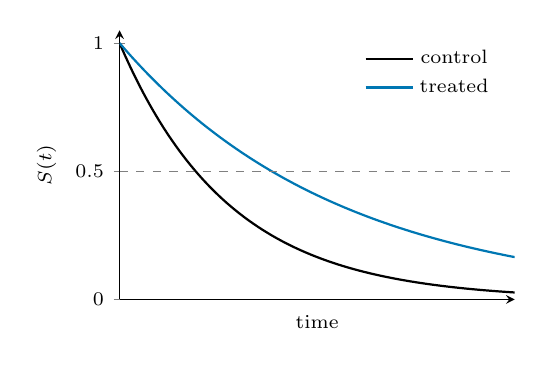
\begin{tikzpicture}
\begin{axis}[
  width=6.6cm, height=5cm,
  xlabel={time}, ylabel={$S(t)$},
  xmin=0, xmax=12, ymin=0, ymax=1.05,
  xtick=\empty, ytick={0,0.5,1},
  legend pos=north east,
  legend style={font=\scriptsize, draw=none},
  axis lines=left,
  tick label style={font=\scriptsize},
  label style={font=\scriptsize},
]
\addplot[domain=0:12, samples=200, thick, black]    {exp(-0.30*x)};
\addlegendentry{control}
\addplot[domain=0:12, samples=200, thick, myaccent] {exp(-0.15*x)};
\addlegendentry{treated}
\draw[dashed, gray] (axis cs:0,0.5) -- (axis cs:12,0.5);
\end{axis}
\end{tikzpicture}
\end{column}
\end{columns}
\end{frame}


%---------------------------------------------------------
\begin{frame}{Why ``horseshoe''? The shrinkage weight}
\begin{columns}[T,onlytextwidth]
\begin{column}{0.5\textwidth}
\vspace{0.3cm}
Reparametrise $\kappa_\ell = 1/(1+\lambda_\ell^2\gamma^2)\in[0,1]$. The posterior mean is
$\widehat\theta = (1-\kappa_\ell)\,\bar y$, and under the horseshoe
\[
\kappa_\ell \sim \mathrm{Beta}\!\left(\tfrac12,\tfrac12\right).
\]
The U-shape puts mass at the extremes:
\begin{itemize}
  \item $\kappa_\ell \approx 0$: signal (no shrinkage).
  \item $\kappa_\ell \approx 1$: noise (full shrinkage).
\end{itemize}
{\footnotesize (van der Pas et al., 2014, 2017: near-minimax contraction.)}
\end{column}
\begin{column}{0.5\textwidth}
\centering
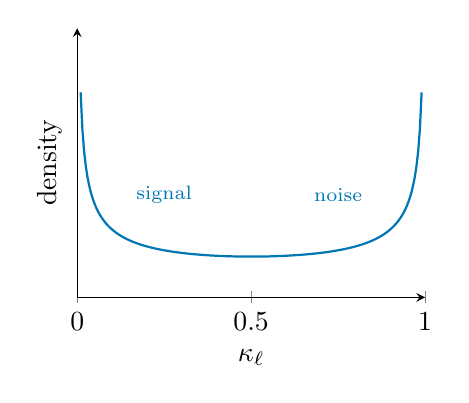
\begin{tikzpicture}
\begin{axis}[
  width=6cm, height=5cm,
  xlabel={$\kappa_\ell$}, ylabel={density},
  xmin=0, xmax=1, ymin=0, ymax=4.2,
  ytick=\empty, xtick={0,0.5,1}, axis lines=left,
]
\addplot[domain=0.01:0.99, samples=200, thick, myaccent]
  {1 / (3.14159 * sqrt(x*(1-x)))};
\node[font=\scriptsize, text=myaccent] at (axis cs: 0.25, 1.6) {signal};
\node[font=\scriptsize, text=myaccent] at (axis cs: 0.75, 1.6) {noise};
\end{axis}
\end{tikzpicture}
\end{column}
\end{columns}
\end{frame}

%---------------------------------------------------------
\begin{frame}{PDAC: the data}
\begin{columns}[T,onlytextwidth]
\begin{column}{0.42\textwidth}
\vspace{0.3cm}
\textbf{TCGA-PAAD cohort:}
\begin{itemize}
  \item $n=110$ resected patients (6-month landmark).
  \item $11$ clinical $+\sim\!3{,}000$ gene expressions.
  \item Censoring $\approx 47\%$; median follow-up $23.3$ mo.
\end{itemize}
\bigskip
\textbf{Treatment:} adjuvant radiotherapy.
\end{column}
\begin{column}{0.58\textwidth}
\centering
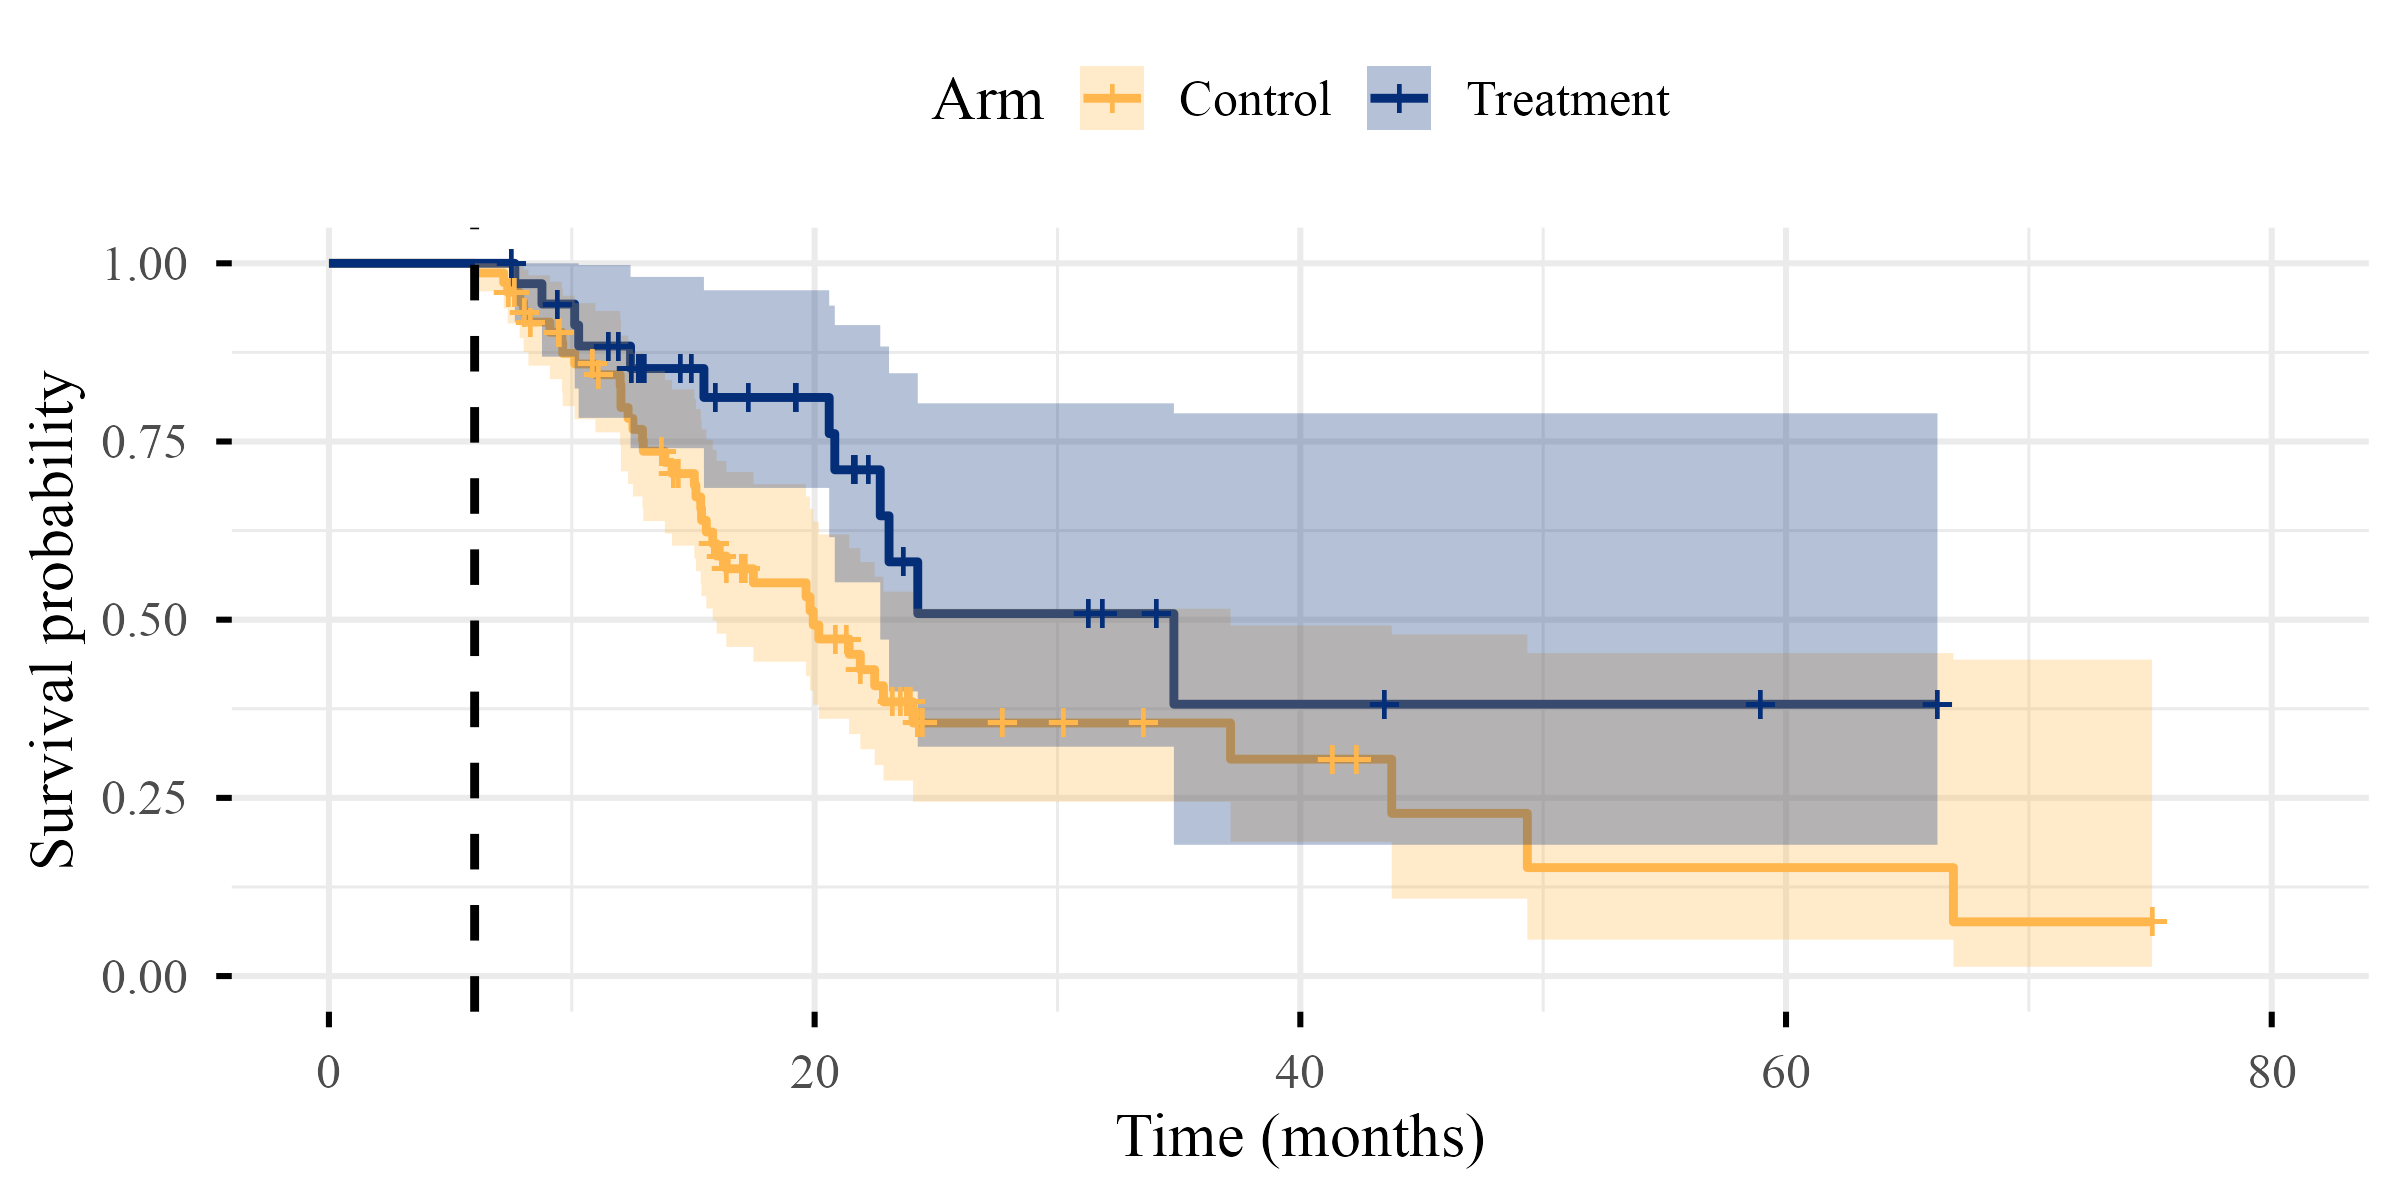
\includegraphics[width=\linewidth]{KM_Landmark.png}
\end{column}
\end{columns}
\end{frame}

%---------------------------------------------------------
\begin{frame}{Censoring via data augmentation}
We follow Tanner \& Wong (1987): treat censored event times as latent variables.
At iteration $t$, for each censored $i$,
\[
\log T_i^{(t)} \sim \N\!\bigl(\hat\mu_i^{(t)},\,\sigma^{2,(t)}\bigr)
\quad\text{truncated to }(\log Y_i,\infty),
\]
with $\hat\mu_i^{(t)} = f^{(t)}(x_i,\hat e(x_i)) + a_i\,\tau^{(t)}(x_i)$.

\bigskip
\textbf{Propensity score:} estimated separately with a binary-outcome Horseshoe Forest (probit augmentation), then plugged into $f$. Avoids feedback (Zigler, 2016); improves finite-sample bias (Hahn et al., 2020).
\end{frame}

%---------------------------------------------------------
\begin{frame}{Simulation 1: data-generating process}
$n=200$, censoring $\approx 35\%$, $p$ swept from $50$ to $5000$:
\[
X_i \sim \mathcal{U}[0,1]^p,\quad A_i\sim\mathrm{Ber}(e(x_i)),\quad
\log T_i \sim \N\!\bigl(f(x_i)+A_i\tau(x_i),\,\sigma^2\bigr).
\]
$e(x_i)=\Phi(-0.5+0.4x_{i1}-0.1x_{i3}+0.3x_{i5})$; $\;f(x_i)=\beta_f^\top x_i$ with $\beta_f$ spike-and-slab.

\smallskip
\textbf{Treatment effect.} Friedman non-linear core $+$ sparse main $+$ sparse interactions,
\[
\tau(x_i)=10\sin(\pi x_{i1}x_{i2})+20(x_{i3}-0.5)^2+10x_{i4}+5x_{i5}+\beta_\tau^\top x_i + x_i^\top\Gamma x_i,
\]
with $\beta_\tau$ spike-and-slab ($s_{\mathrm{main}}=0.05$) and sparse symmetric $\Gamma$ ($s_{\mathrm{int}}=0.01$).
\end{frame}

%---------------------------------------------------------
\begin{frame}{Simulation 2: data-generating process}
$p=500$, $n=100$, $|S|=5$ strong confounders, $|W|\in\{1,\ldots,20\}$ weak confounders:
\begin{align*}
e(x_i)    &\propto \tfrac{1}{\sqrt{5+|W|}}\Bigl(\textstyle\sum_{j\in S} x_{ij} + 2\sum_{j\in W} x_{ij}\Bigr),\\
f(x_i)    &= 4\sum_{j\in S} x_{ij} + \sum_{j\in W} x_{ij},\\
\tau(x_i) &= 1 + \sum_{j\in S}\beta_j\,x_{ij}.
\end{align*}
\end{frame}

%---------------------------------------------------------
\begin{frame}{Full conditional update of step heights}
Given the current tree $\T$ with $L$ leaves, encode the partition by $D\in\R^{n\times L}$. The conditional posterior of $h\in\R^L$ is
\[
h \sim \N_L\!\Bigl(\Omega^{-1}D^\top R,\;\Omega^{-1}\Bigr),\qquad
\Omega = D^\top D + \bigl(\omega\gamma^2\,\mathrm{diag}(\lambda_1^2,\ldots,\lambda_L^2)\bigr)^{-1}.
\]
Coordinate-wise,
\[
h_\ell\mid\cdot \;\sim\;
\N\!\left(\tfrac{\bar R_\ell}{n_\ell+1/(\gamma^2\lambda_\ell^2\omega)},\;
          \tfrac{\sigma^2}{n_\ell+1/(\gamma^2\lambda_\ell^2\omega)}\right).
\]
The shrinkage parameters update in closed form via the inverse-gamma auxiliary representation (Makalic \& Schmidt, 2016).
\end{frame}

%---------------------------------------------------------
\begin{frame}{Sparsity on splits can drop real signal}
\textbf{Setup.} $n=500$, $p=10$; first 5 covariates carry strong signal, rest are noise. Three independent replications shown.

\begin{figure}
\centering
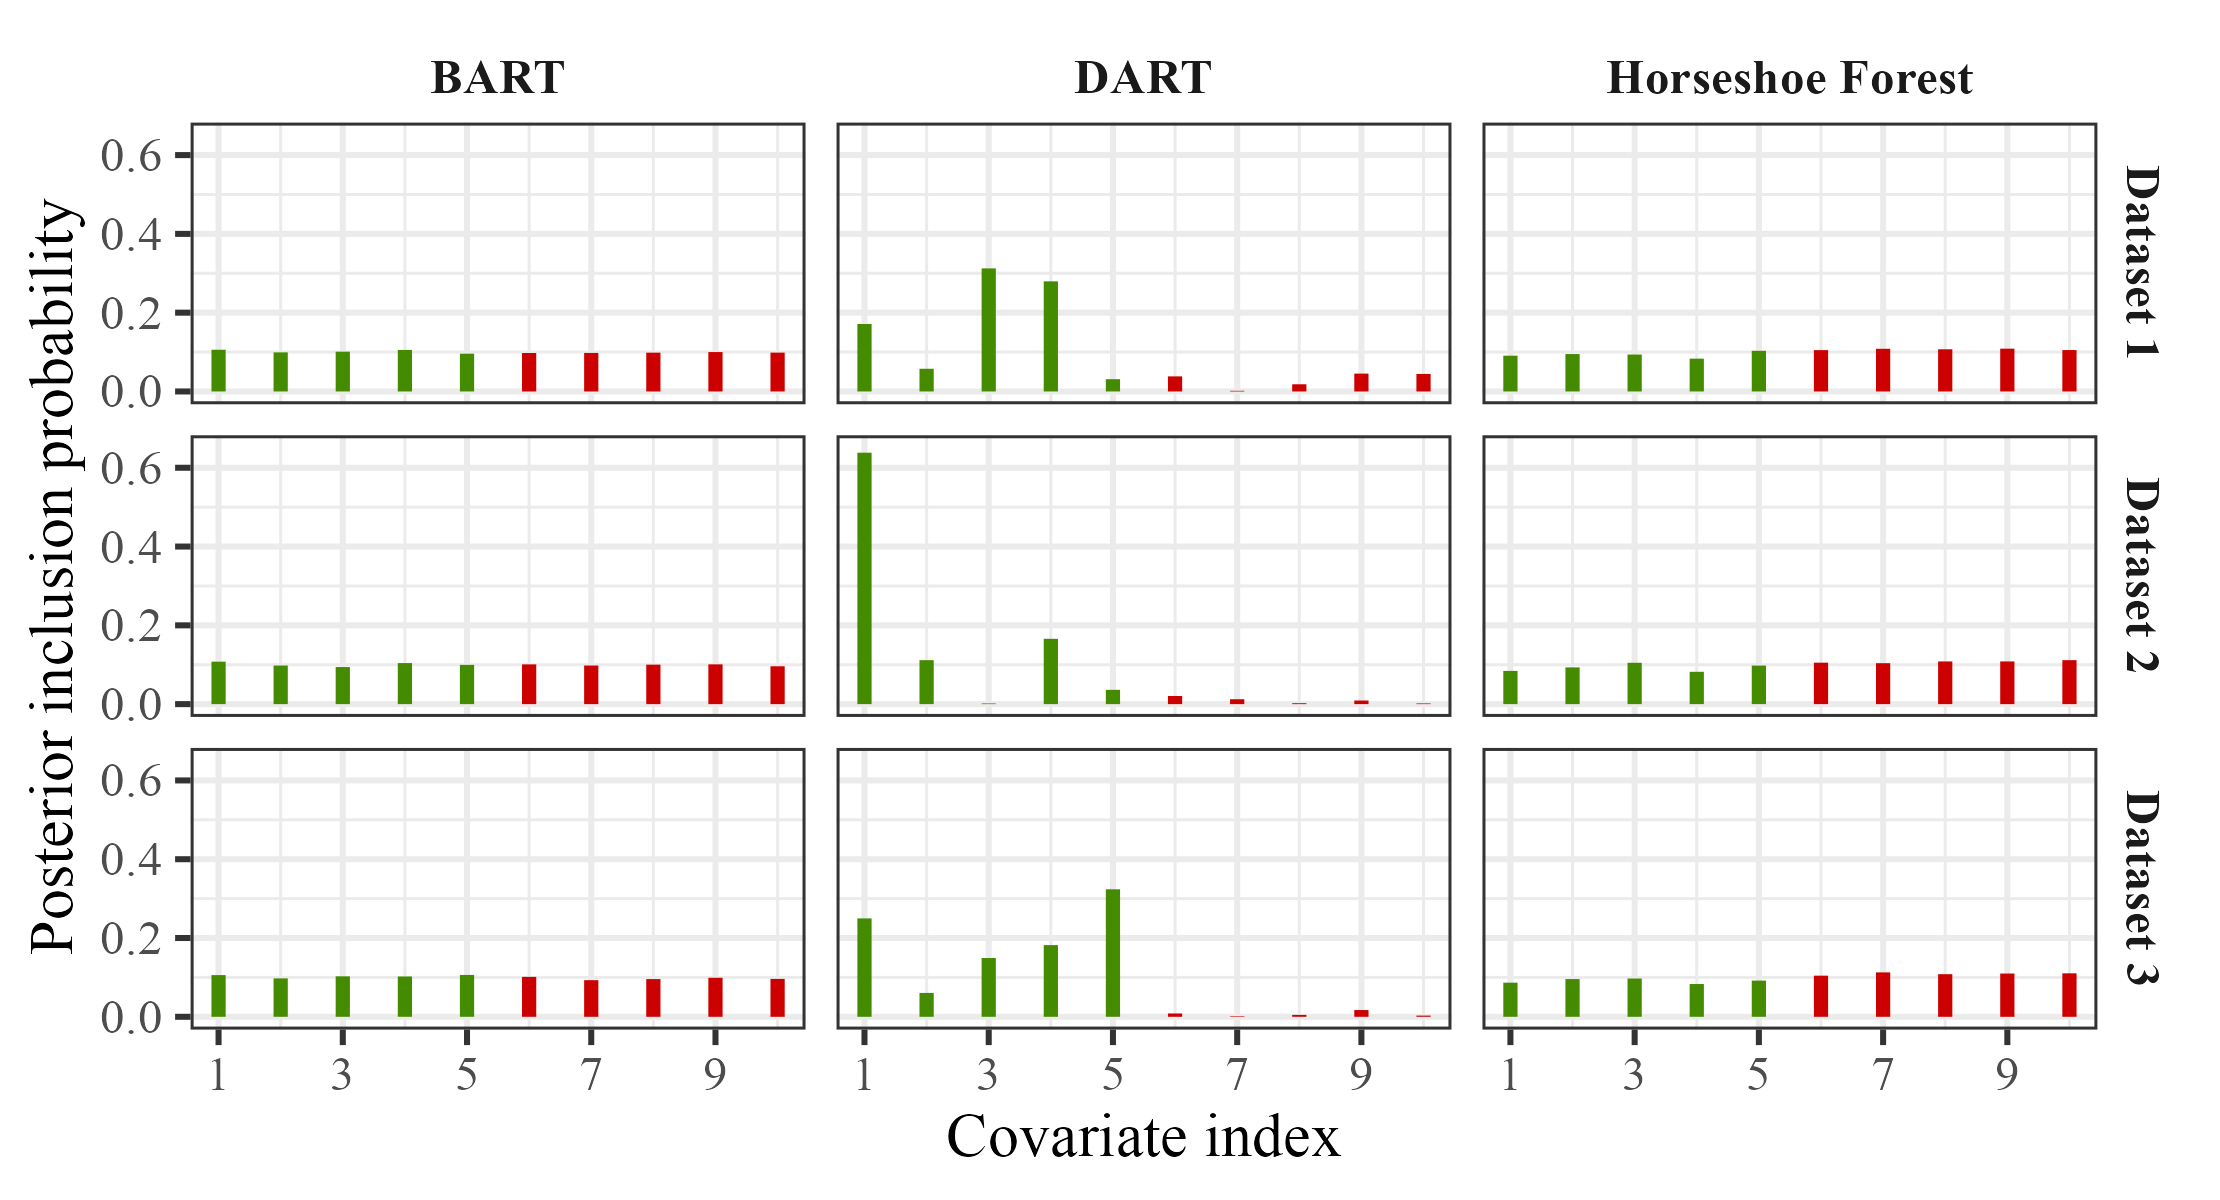
\includegraphics[width=0.85\linewidth]{revision_posterior_inclusion_plot.png}
\end{figure}
\end{frame}

\end{document}
